\documentclass{beamer}

\usepackage[beamer]{shortcut}
\usepackage{bibentry}


\def\TikzLocation{./tikz/}
\def\tkzscl{1}

\graphicspath{{./images/}}
\usepackage[square]{natbib}



% \definecolor{linkcolor}{RGB}{45,163,65}
\definecolor{Z}{RGB}{45,162,65}
\definecolor{D}{RGB}{180,35,35}
\def\varX{{\color{D} \pmb x}}
\def\varZ{{\color{linkcolor} \pmb z}}
\def\varD{{\color{Z} \pmb G}}

% Dark-red for citations and linkcolor for contributions
\hypersetup{
	citecolor=darkred
}
\definecolor{contribcolor}{RGB}{83,83,182}


\author{Thomas Moreau}
\institute{\\ INRIA Saclay - MIND Team}
\title{
	A Journey through Algorithm Unrolling for Inverse Problems
}

\setbeamertemplate{title page}[frame]
\def\extraLogo{}

\begin{document}

\begin{frame}
	\titlepage
    \nobibliography{library.bib}
\end{frame}



% \frame{
%     \frametitle{Context: functional Neuroimaging}

%     \large {\bf Goal:}
%     Study the brain mechanisms while it is functioning.\\[3em]

%     {\bf Outputs:}\\[1em]
%     \begin{itemize}\itemsep1em
%         \item {\bf Functional Atlases:} Link areas of the brain to specific cognitive functions.
%         \item {\bf Functional Connectivity:} Highlight the information flow in the brain.
%         \item {\bf Healthcare:} Develop bio-markers for neurological disorders.
%     \end{itemize}
% }

% \frame[t]{
%     \frametitle{Context: functional Neuroimaging}

%     {\large How to record living brains electrical activity: \textbf{Electrophysiology}}\\[.3em]

%     \centering\large Direct measurement: intracranial EEG.\\[.5em]
%         \centering
%         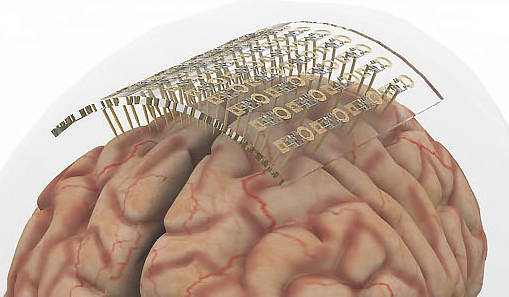
\includegraphics[width=.7\textwidth]{brain_probe.jpg}\\[1em]
%         \begin{columns}
%             \techterm{\color{darkblue} High Localization}%
%             \techterm{Low Resolution}%
%             \techterm{Invasive}%
%         \end{columns}
% }


% \frame[t]{
%     \frametitle{Context: functional Neuroimaging}

%     {\large How to record living brains electrical activity: \textbf{Electrophysiology}}\\[.3em]

%     \large\centering Remote measurement: M/EEG.\\[-.5em]
%     \begin{columns}[T]
%         \column{.35\textwidth}
%         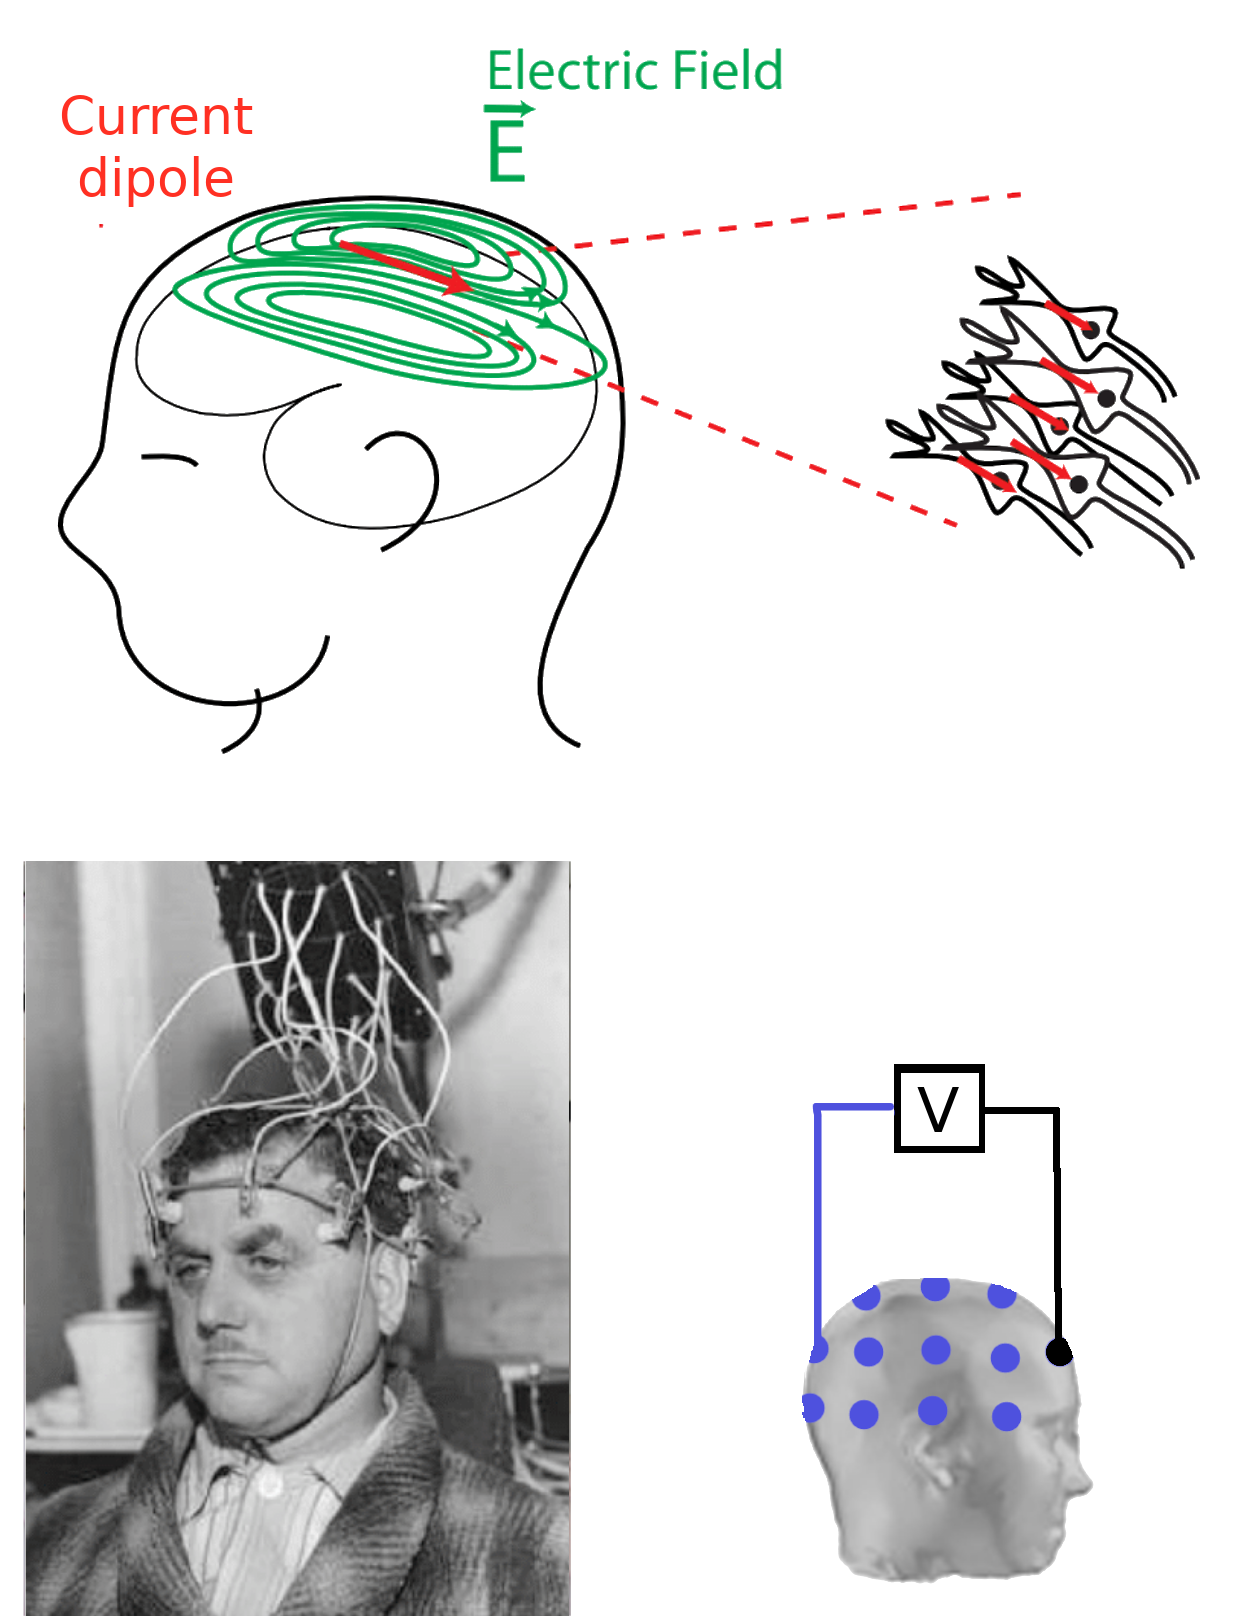
\includegraphics[width=\textwidth]{eeg_presentation}
%         \column{.35\textwidth}
%         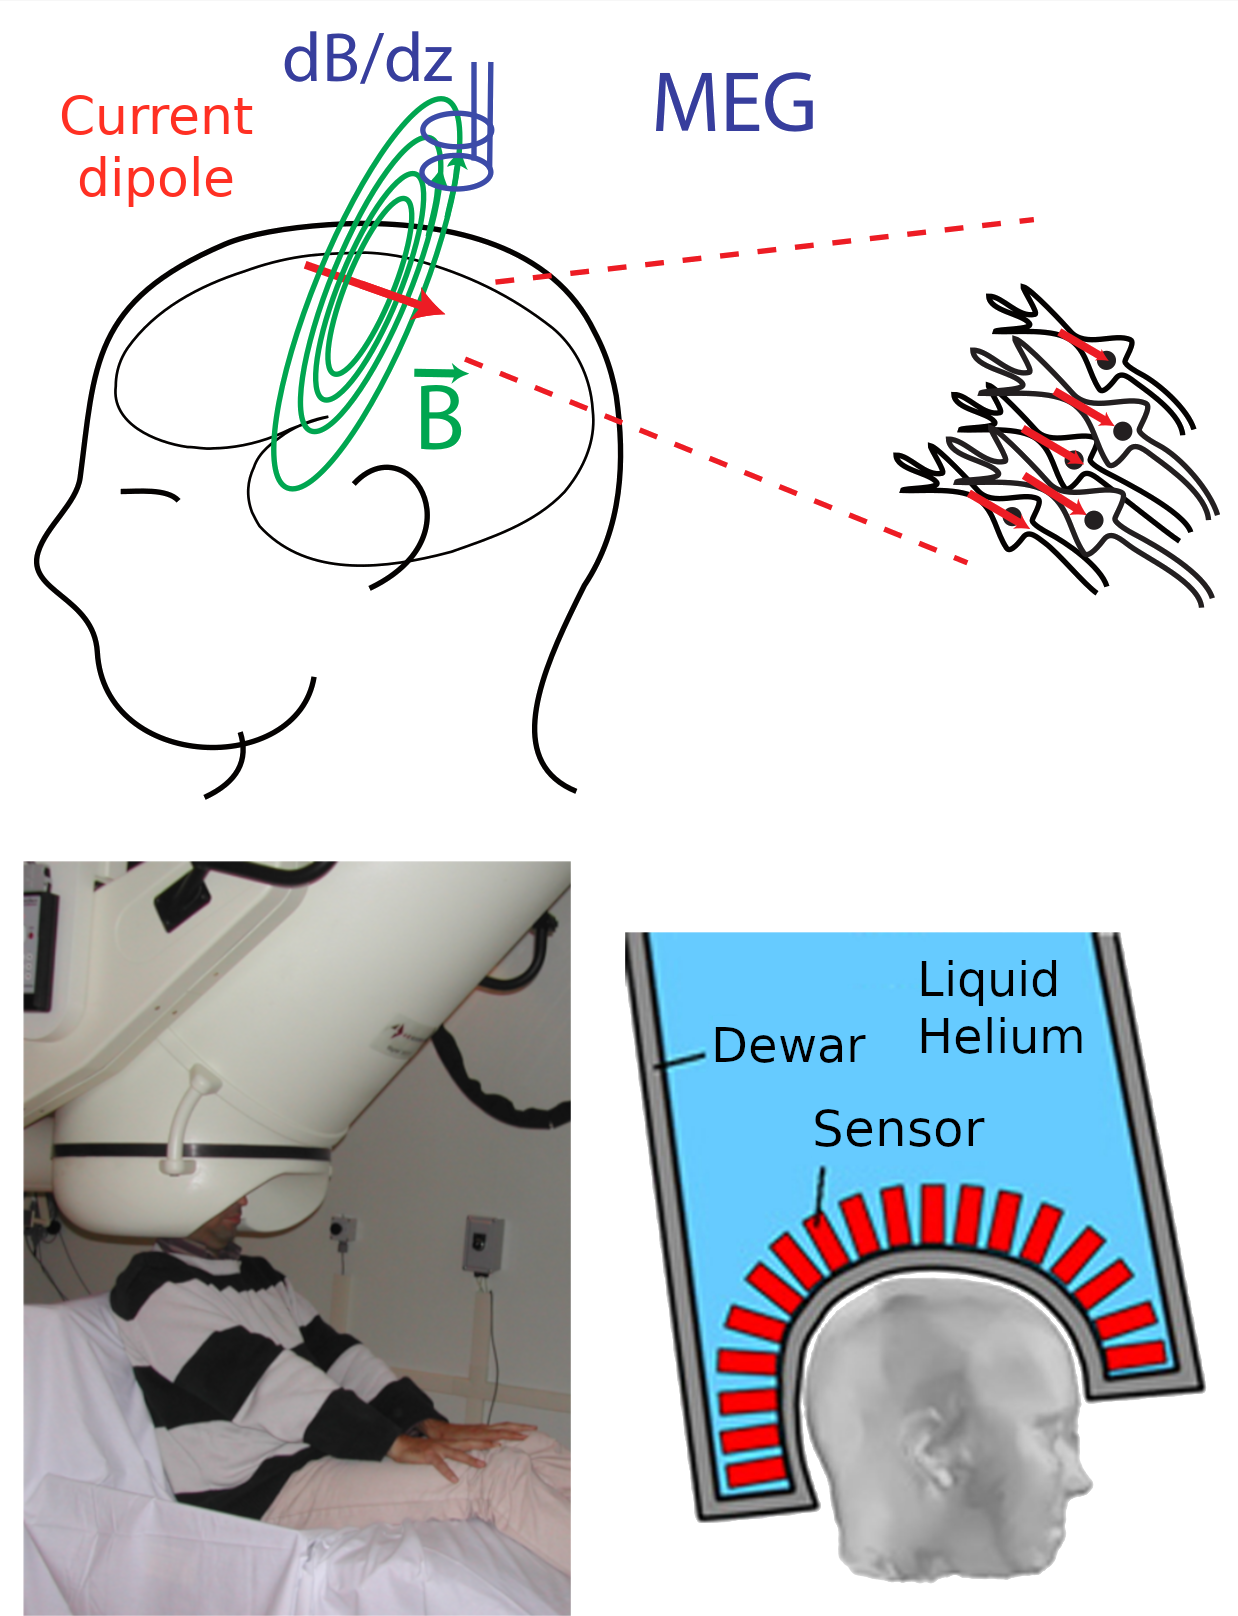
\includegraphics[width=\textwidth]{meg_presentation}
%     \end{columns}
%     % \only<2>{
%     \begin{columns}
%         \techterm{No Localization}%
%         \techterm{\color{darkblue} Global}%
%         \techterm{\color{darkblue} Non Invasive}%
%     \end{columns}
%     % }

% }

% \frame{
%     \frametitle{M/EEG signals}

%     {\Large\bf Multivariate time-series $x$}\\[1em]

%     \centering
%     \alt<3>{
%         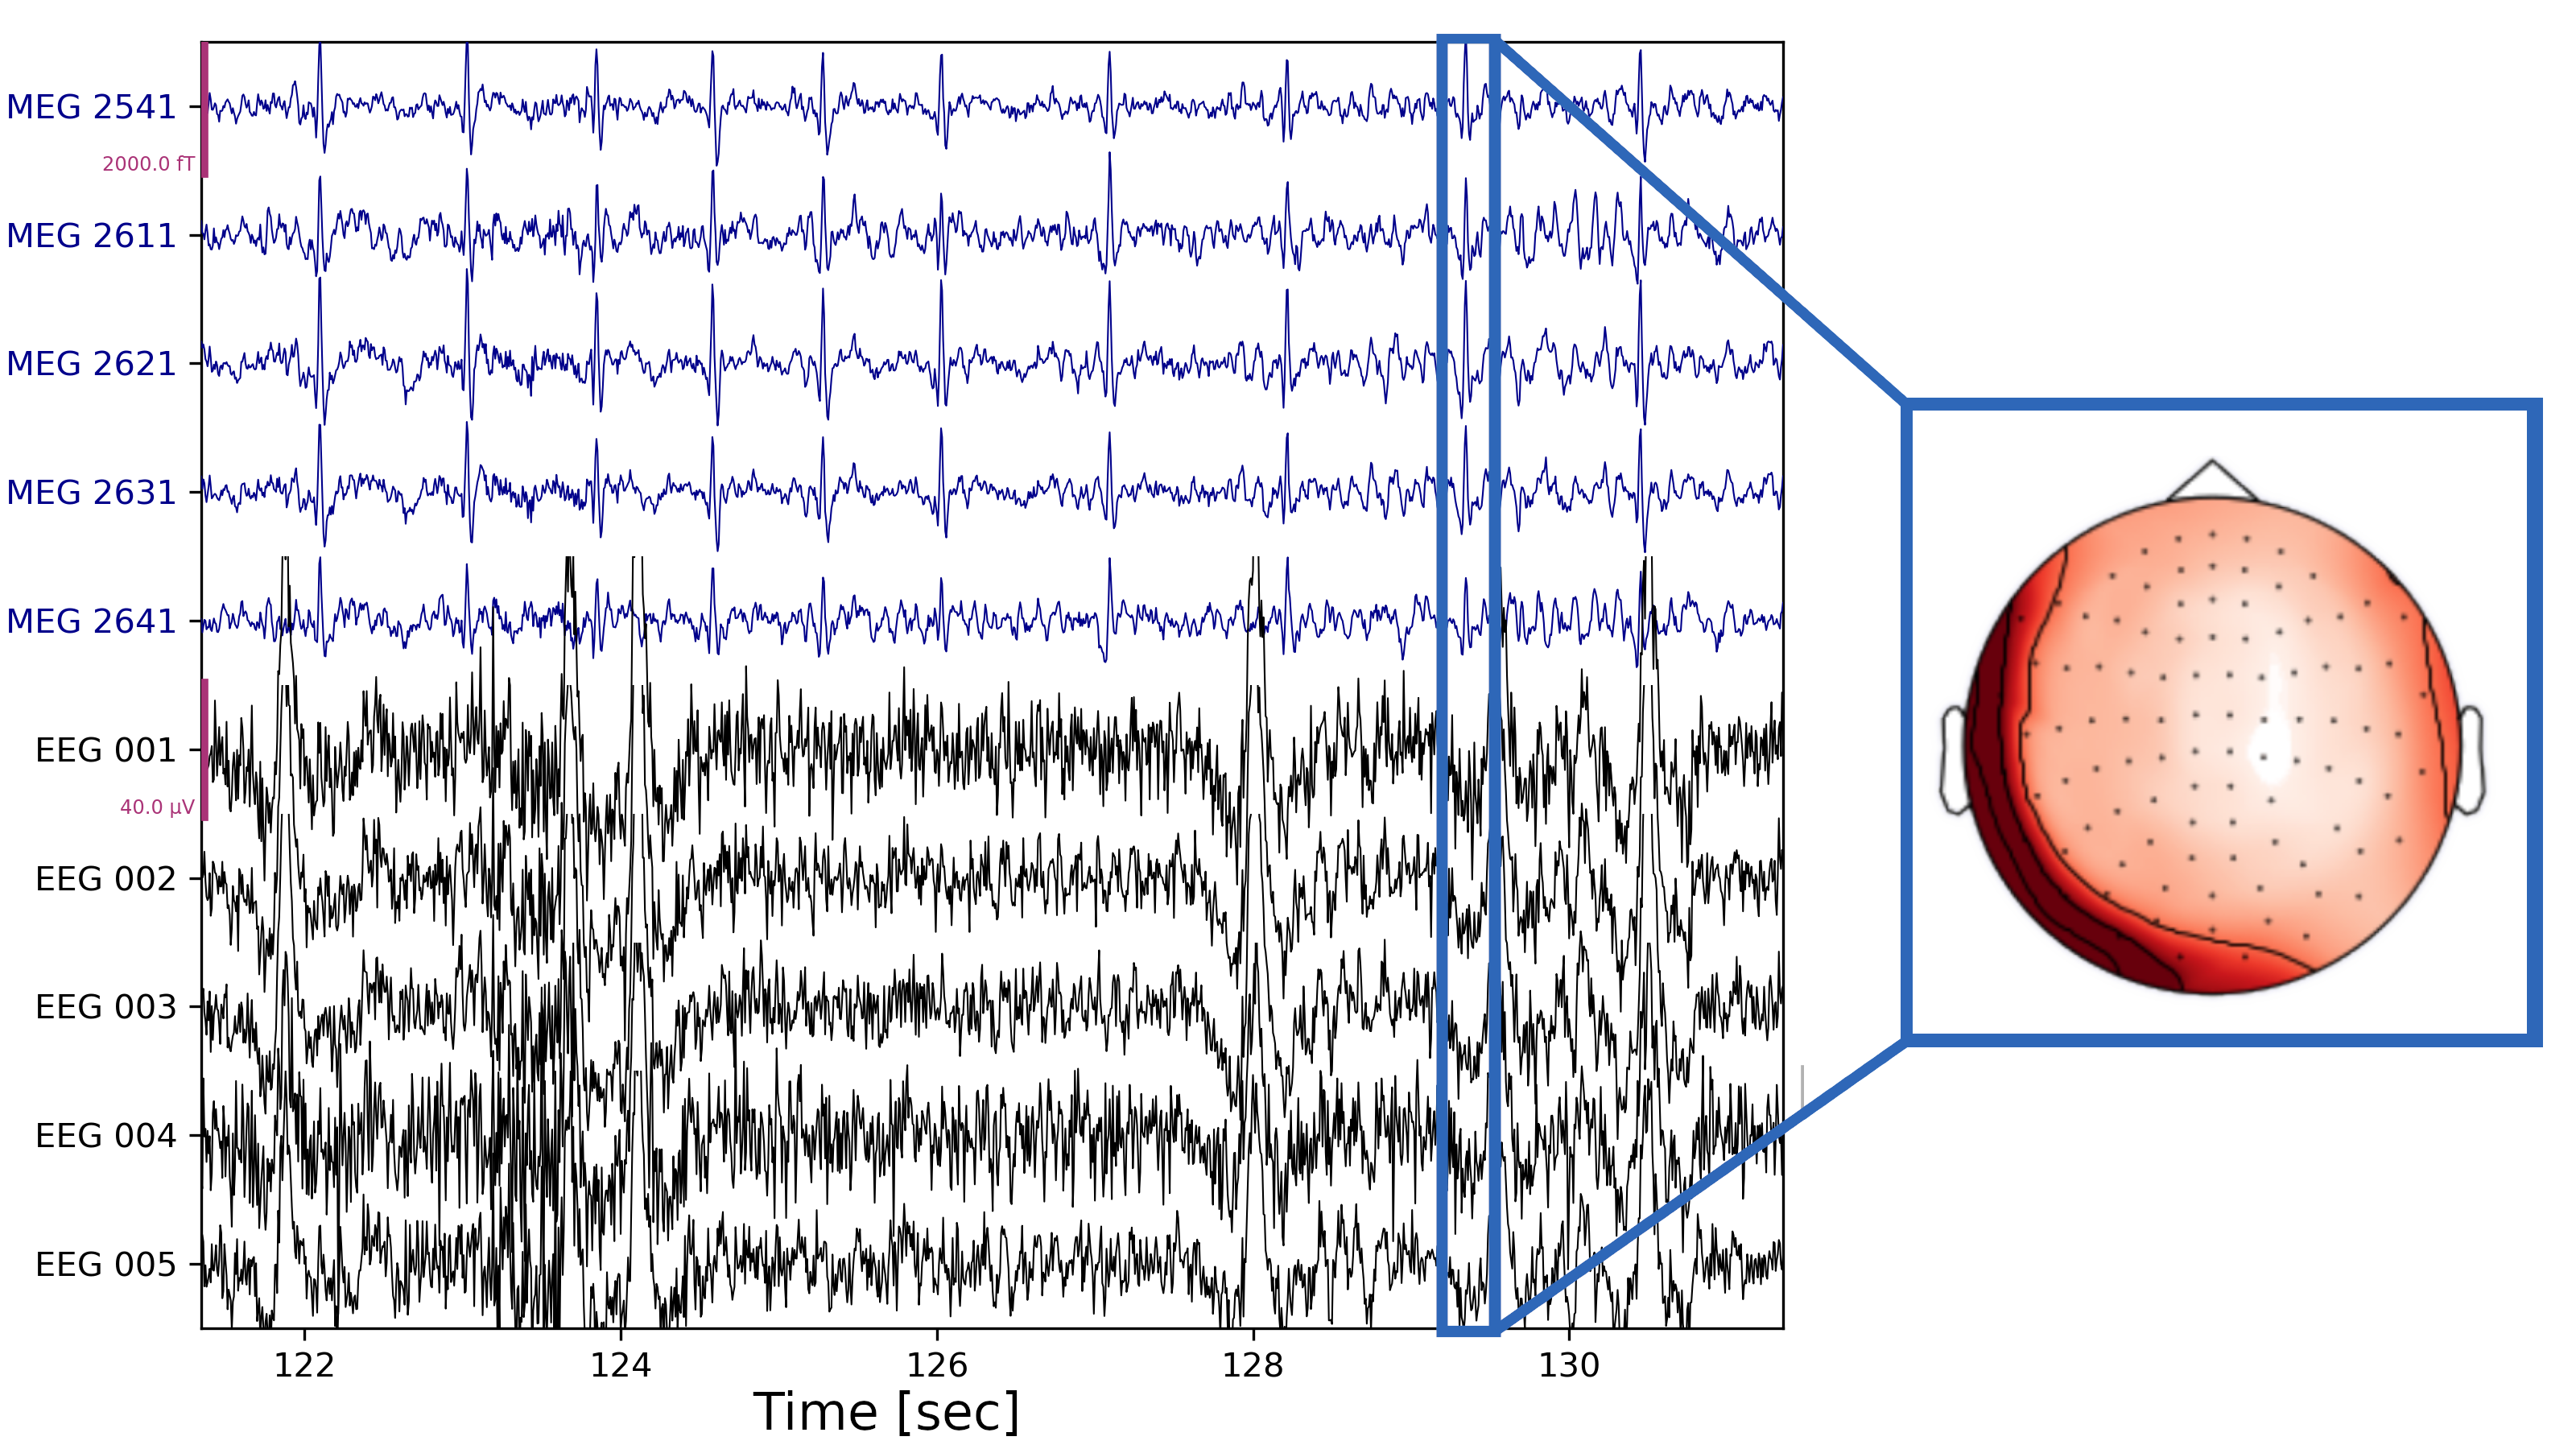
\includegraphics[width=.9\textwidth]{meeg_data_highlight}
%     }{
%         \alt<1>{
%             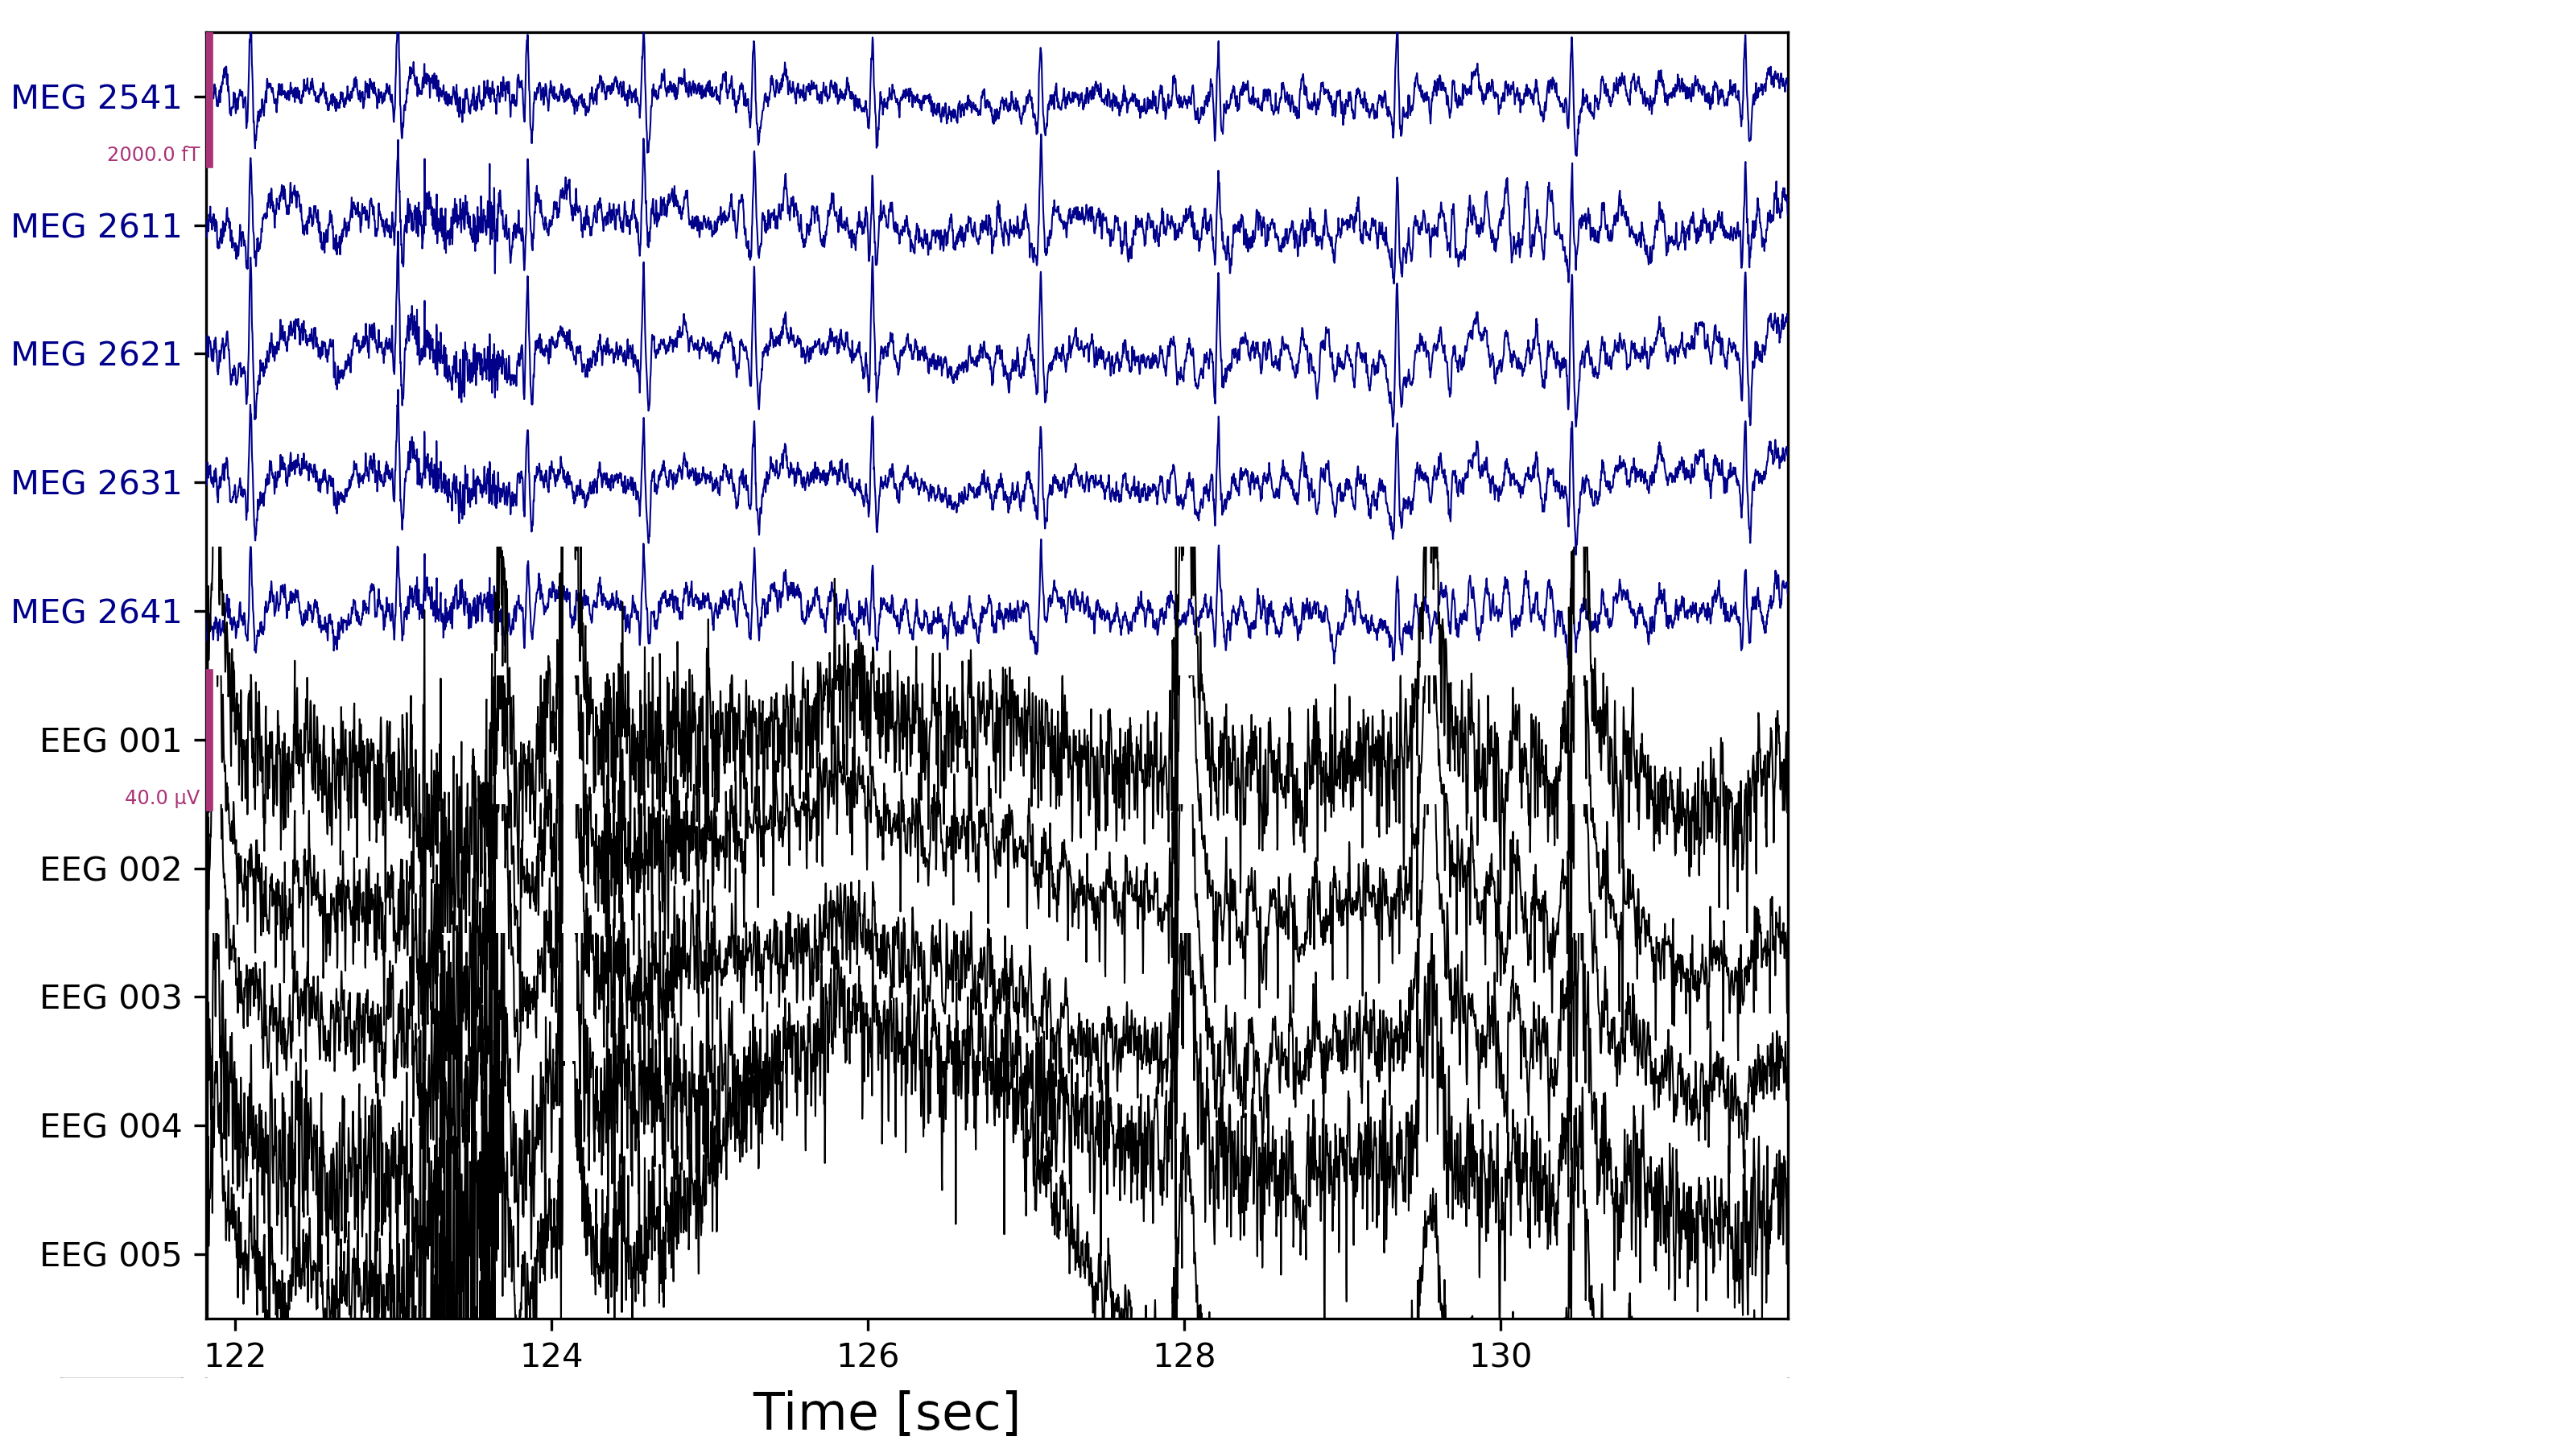
\includegraphics[width=.9\textwidth]{meeg_data}
%         }{
%             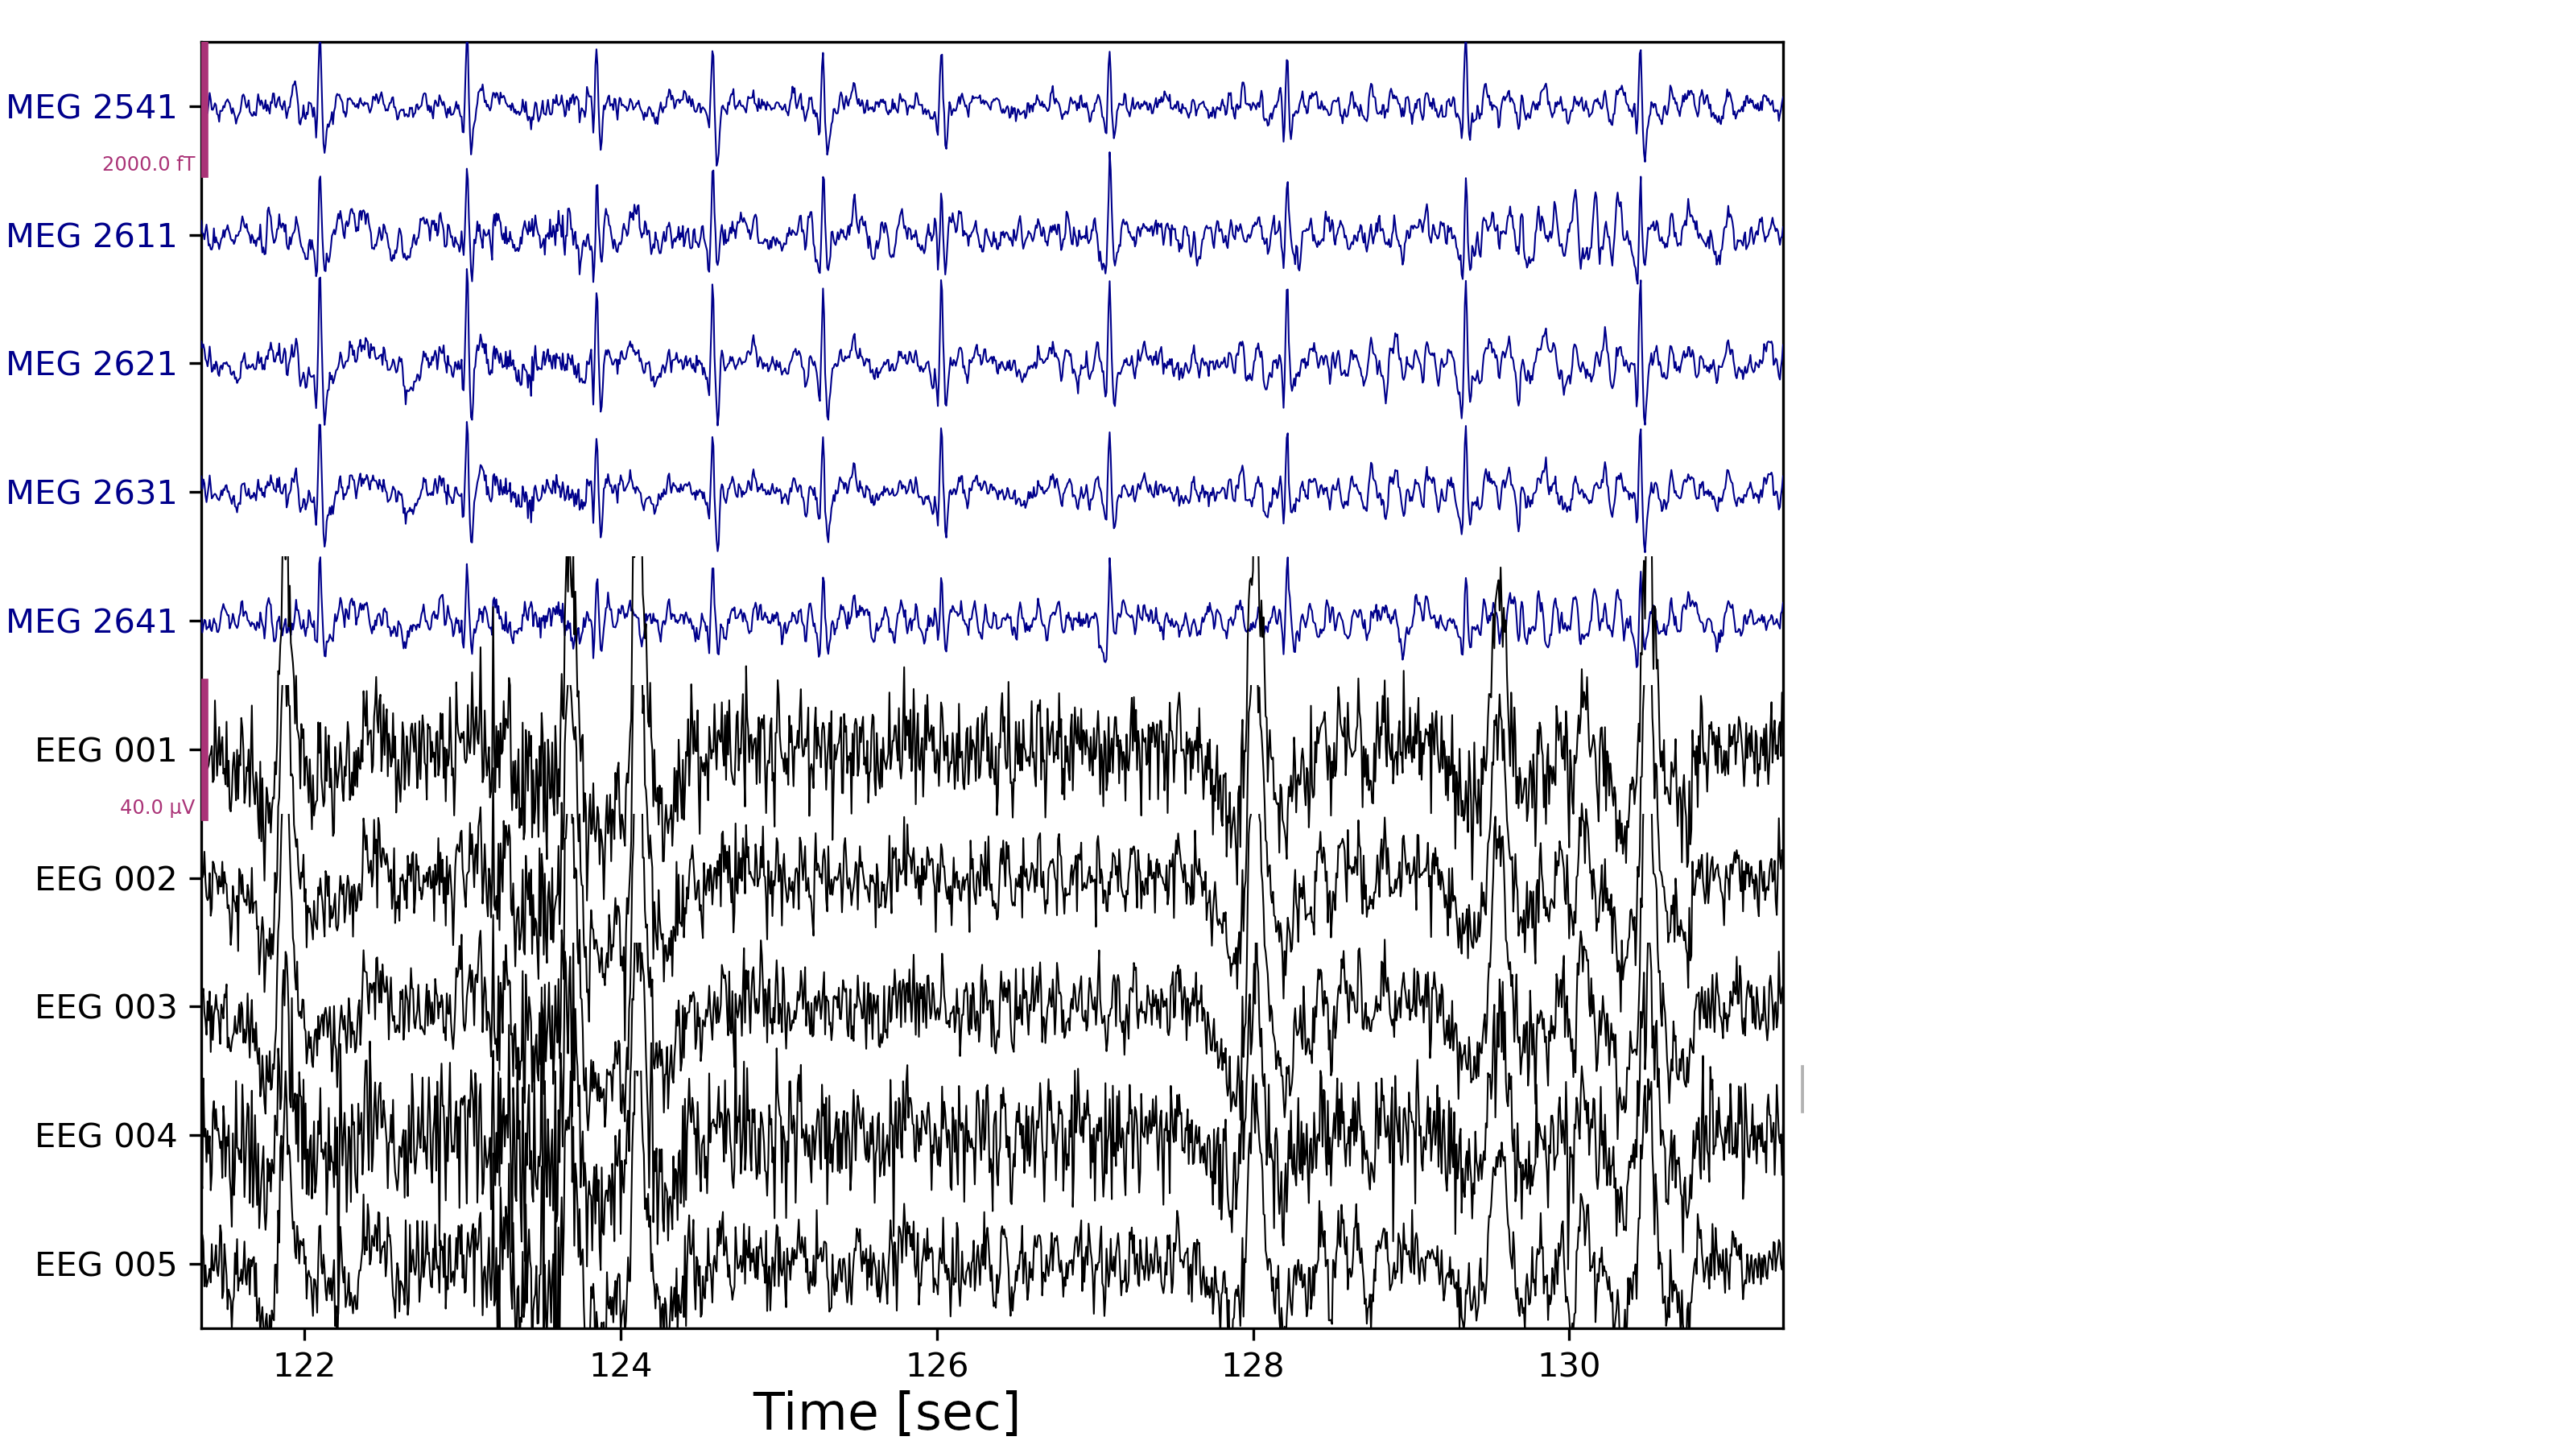
\includegraphics[width=.9\textwidth]{meeg_data_preproc}
%         }
%     }\\[1em]
%     \begin{columns}
%         \techterm{Noisy}%
%         \techterm{Many artifacts}%
%         \techterm{Complex}%
%     \end{columns}
% }

\frame[t]{
    \frametitle{Inverse Problems}

    \vskip-1em
    \begin{columns}[T]

        \column{.5\textwidth}
            {\bf Neuroimaging -- M/EEG}\\[.5em]
            {\centering
            \begin{tikzpicture}
            \tikzset{
                %Define standard arrow tip
                >=stealth',
                %Define style for boxes
                varstyle/.style={
                    rectangle,
                    rounded corners,
                    draw=black,
                    text width=1em,
                    minimum height=1.5em,
                    text centered},
                small/.style={
                    font=\footnotesize,
                }
            }
            \node (meg) {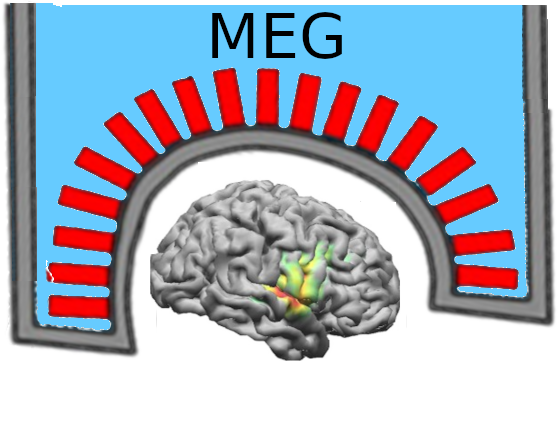
\includegraphics[width=6em]{meg_localised_source}};
            \draw[->, thick] (meg.east) -- ++(6em, 0)
            node[midway, align=center,small] (maxwell) {Maxwell's\\Equations}
            node[right] (topomap) {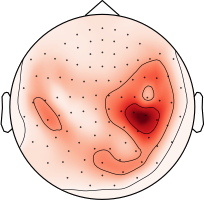
\includegraphics[width=3em]{topomap_somato}};

            \draw[<-, thick] ($(meg.east) + (0, 0.75em)$) to[bend left, looseness=1]
            node [midway, above,small] {Inverse Problem}
            ($(topomap.west) + (0, 0.75em)$);
            \end{tikzpicture}}

            \vskip-.5em
            {\bf Astrophysics}\\[.5em]
            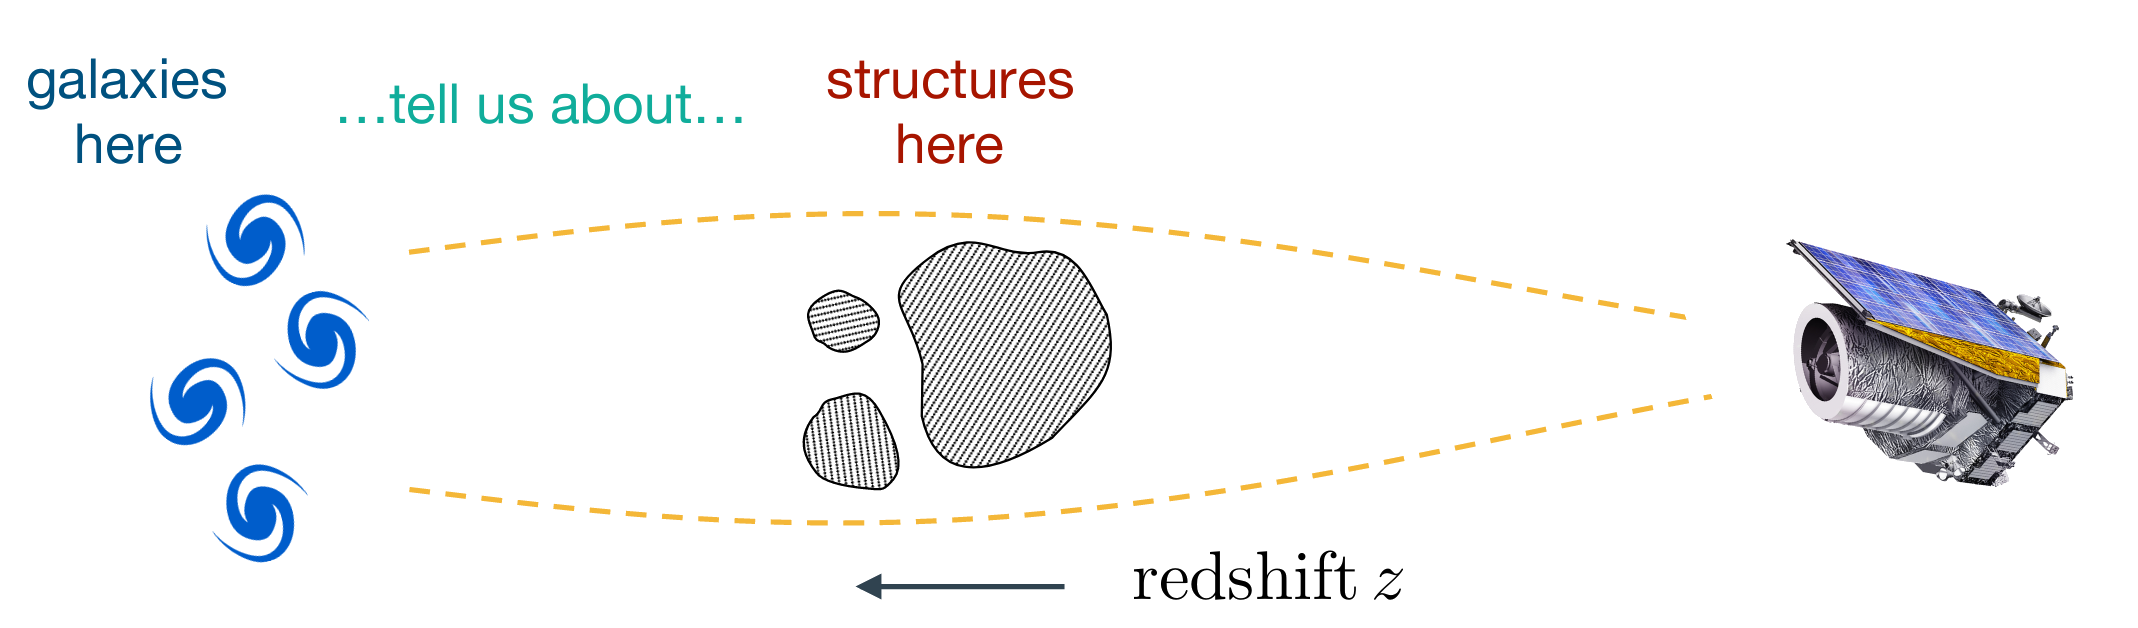
\includegraphics[width=\textwidth]{weak_lensing}\\

            {\bf Seismology -- Prospection}\\[.5em]
            {\centering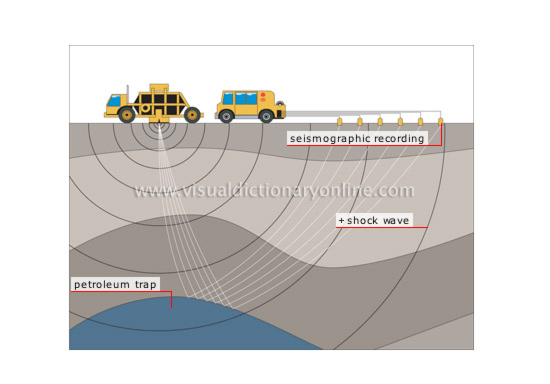
\includegraphics[width=.5\textwidth, trim={6.7em 4em 7em 5em}, clip]{InverseProblem_petroleum}\\}

        \column{.5\textwidth}

            {\bf Neuroimaging -- MRI}\\[1em]
                \begin{columns}[c]
                \column{.5\textwidth}    \centering
                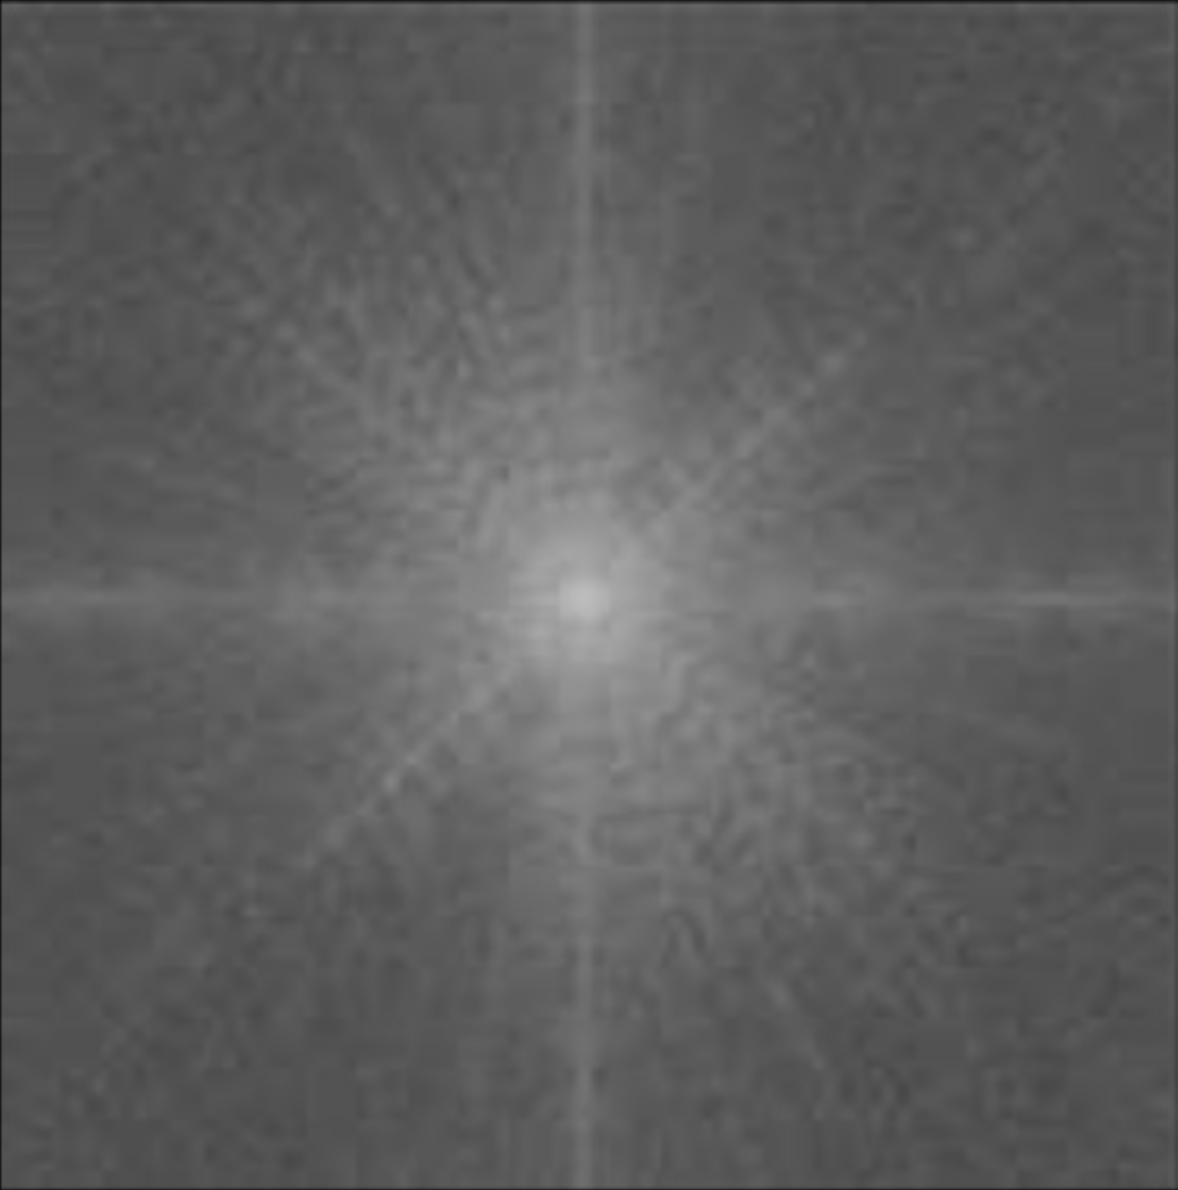
\includegraphics[width=.8\textwidth]{K_space}\\
                \column{.5\textwidth} \centering
                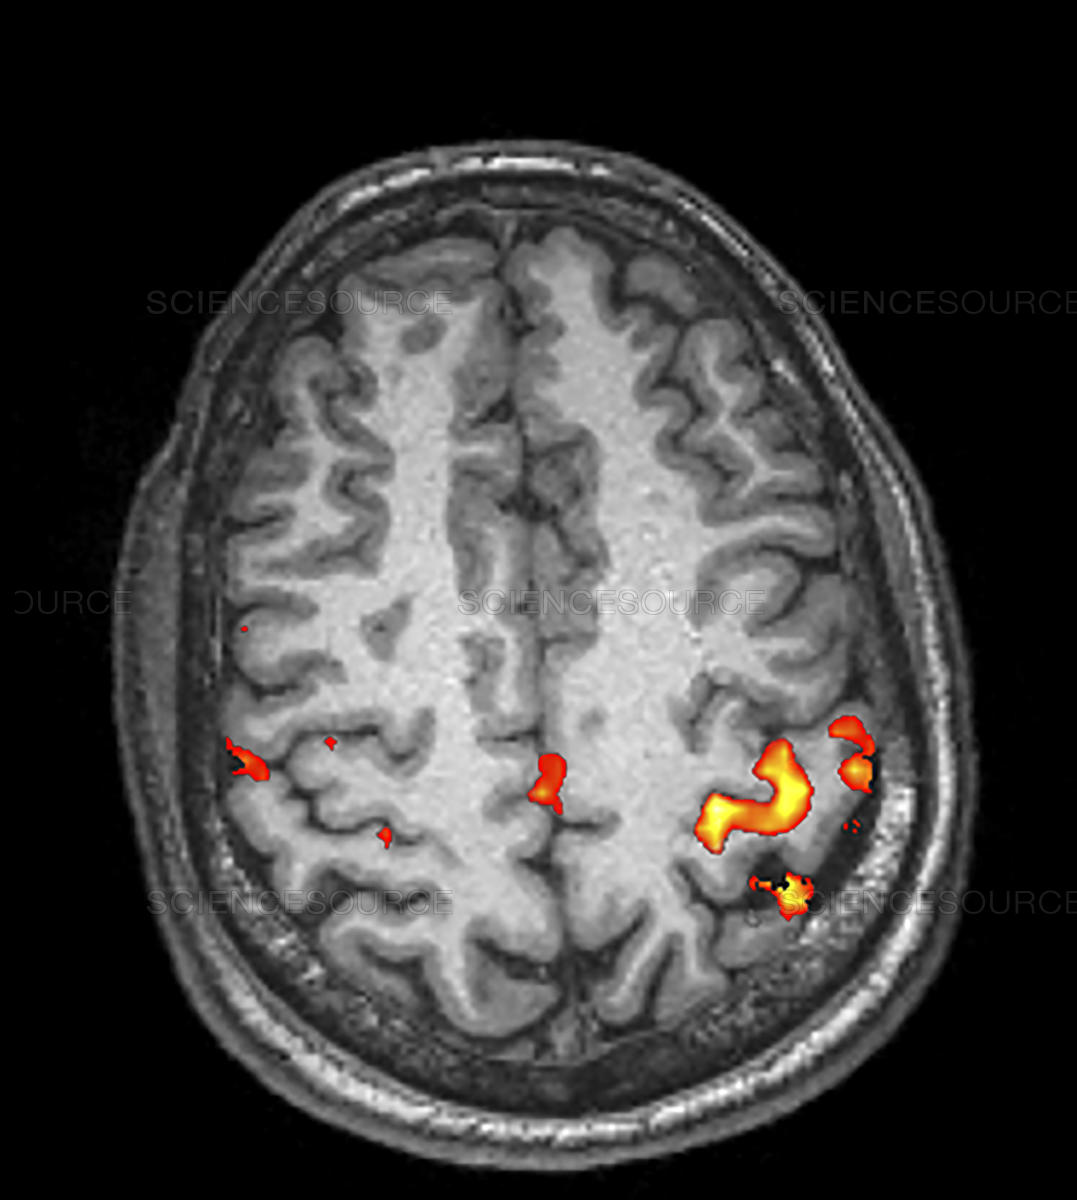
\includegraphics[width=.8\textwidth]{brain_scan}\\
                \end{columns}

            \vskip1.5em
            {\bf Imaging}\\[1em]
            \centering
            \uncovergraphics<1>[width=.8\textwidth, trim={0em 2em 37em 2em}, clip]{super_resolution.png}\\
            Super-Resolution, Inpainting, Deblurring, ...
        \end{columns}

}

\frame{
    \frametitle{Inverse Problem: Source Localization for M/EEG}

    \setbeamercovered{invisible}
    {\centering
    \begin{tikzpicture}
    \tikzset{
        %Define standard arrow tip
        >=stealth',
        %Define style for boxes
        varstyle/.style={
            rectangle,
            rounded corners,
            draw=black,
            text width=1em,
            minimum height=1.5em,
            text centered},
    }
    \node (meg) {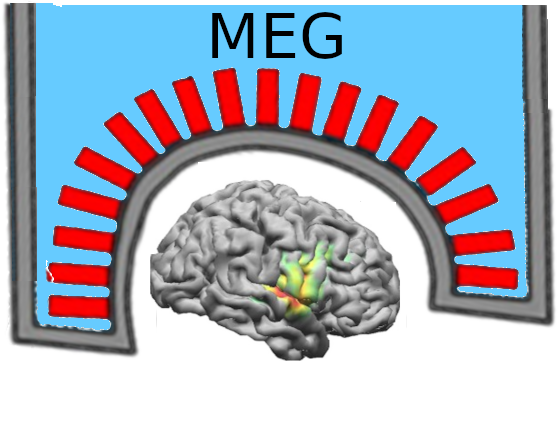
\includegraphics[width=12em]{meg_localised_source}};
    \draw[->, thick] ($(meg.east) - (0, 1.5em)$) -- ++(8em, 0)
    node[midway, align=center] (maxwell) {Maxwell's\\Equations}
    node[right] (topomap) {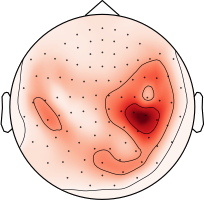
\includegraphics[width=6em]{topomap_somato}};
    \node[varstyle, below=.5em] at (topomap.south) (varX) {$\varX$};
    \node[below=0em of varX.south] {\bf Observed signal};
%        \draw[->, thick] (topomap.east) -- ++(5em, 0)
%        node[midway, align=center] {\small Problème\\ \small inverse}
    \node[varstyle, below=.2em of meg]
        (varZ) {$\varZ$};
        \node[below=0em of varZ.south] {\bf Electrical activity};
    \node[varstyle, below=3.8em of maxwell.center]
        (varD) {$\varD$};

    \uncover<2->{
         \draw[<-, thick] (meg.east) to[bend left, looseness=1]
            node [midway, above] {Inverse Problem}
            ($(topomap.west) + (0, 1.5em)$);
    }
    \end{tikzpicture}}
    \vskip0em
    {\bf Forward model: }$\varX{} = \varD\varZ + \varepsilon$
    \hskip3em
    \uncover<2->{{\bf Inverse problem:} $\varZ = f(\varX)$}\\
    \uncover<3->{
        % \centering
        % \myitem{} Dipole fit
        % \hskip2em
        % \myitem{} Regularized optimization
        % \hskip2em
        % \myitem{} Deep-learning\\
        % \mycite{Sarvas1987}\hskip2em
        % \mycite{Gramfort2012}\hskip2em
        % \mycite{Hecker2021}
        \vskip1em
        \myitem{} Ill-posed problem: many solutions $\varZ$ such that $\varD\varZ=\varX$\\[.5em]
        \myitem{} Noisy problem: need to account for $\varepsilon$
        % Ill-posed and noisy, can amplify the noise: $f(\varX) = \varZ + \varD^\dagger\varepsilon$
    }

}

\frame[t]{
    \frametitle{Inverse Problems}

    \vskip-1em
    \begin{columns}[T]

        \column{.5\textwidth}
            {\bf Neuroimaging -- M/EEG}\\[.5em]
            {\centering
            \begin{tikzpicture}
            \tikzset{
                %Define standard arrow tip
                >=stealth',
                %Define style for boxes
                varstyle/.style={
                    rectangle,
                    rounded corners,
                    draw=black,
                    text width=1em,
                    minimum height=1.5em,
                    text centered},
                small/.style={
                    font=\footnotesize,
                }
            }
            \node (meg) {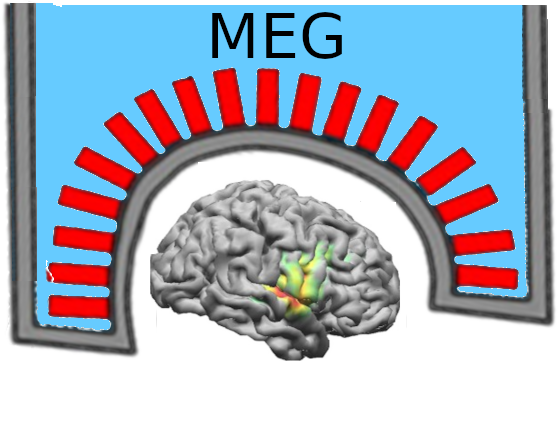
\includegraphics[width=6em]{meg_localised_source}};
            \draw[->, thick] (meg.east) -- ++(6em, 0)
            node[midway, align=center,small] (maxwell) {Maxwell's\\Equations}
            node[right] (topomap) {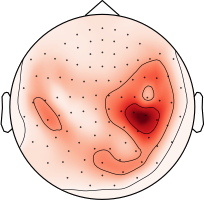
\includegraphics[width=3em]{topomap_somato}};

            \draw[<-, thick] ($(meg.east) + (0, 0.75em)$) to[bend left, looseness=1]
            node [midway, above,small] {Inverse Problem}
            ($(topomap.west) + (0, 0.75em)$);
            \end{tikzpicture}}

            \vskip-.5em
            {\bf Astrophysics}\\[.5em]
            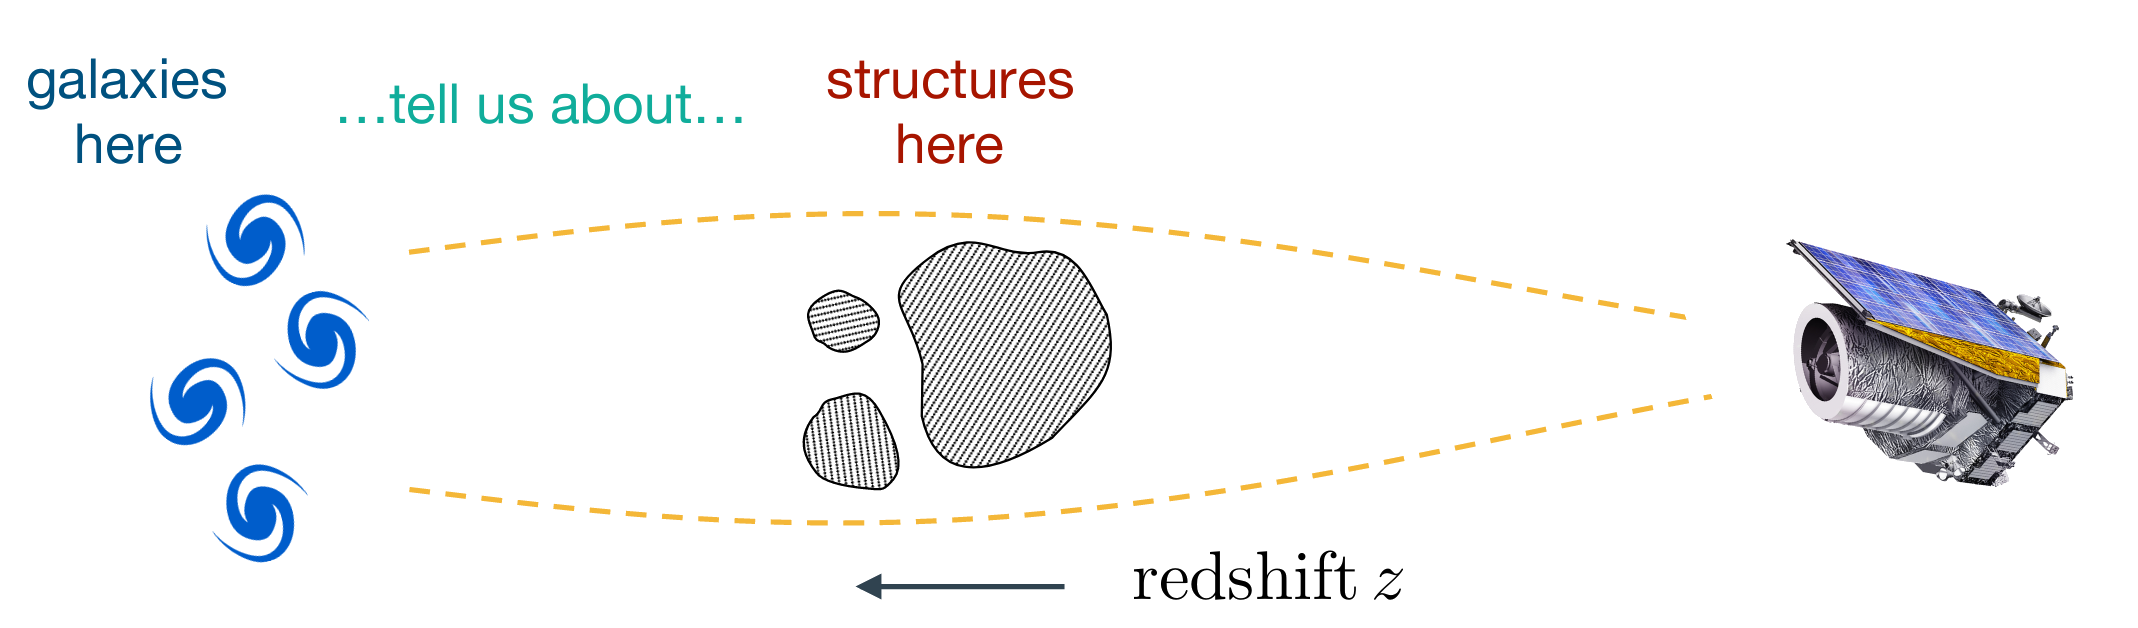
\includegraphics[width=\textwidth]{weak_lensing}\\

            {\bf Seismology -- Prospection}\\[.5em]
            {\centering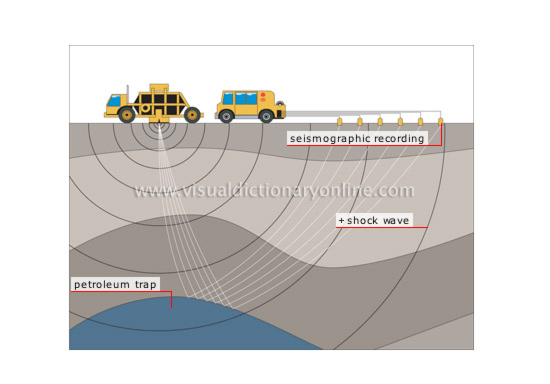
\includegraphics[width=.5\textwidth, trim={6.7em 4em 7em 5em}, clip]{InverseProblem_petroleum}\\}

        \column{.5\textwidth}

            {\bf Neuroimaging -- MRI}\\[1em]
                \begin{columns}[c]
                \column{.5\textwidth}    \centering
                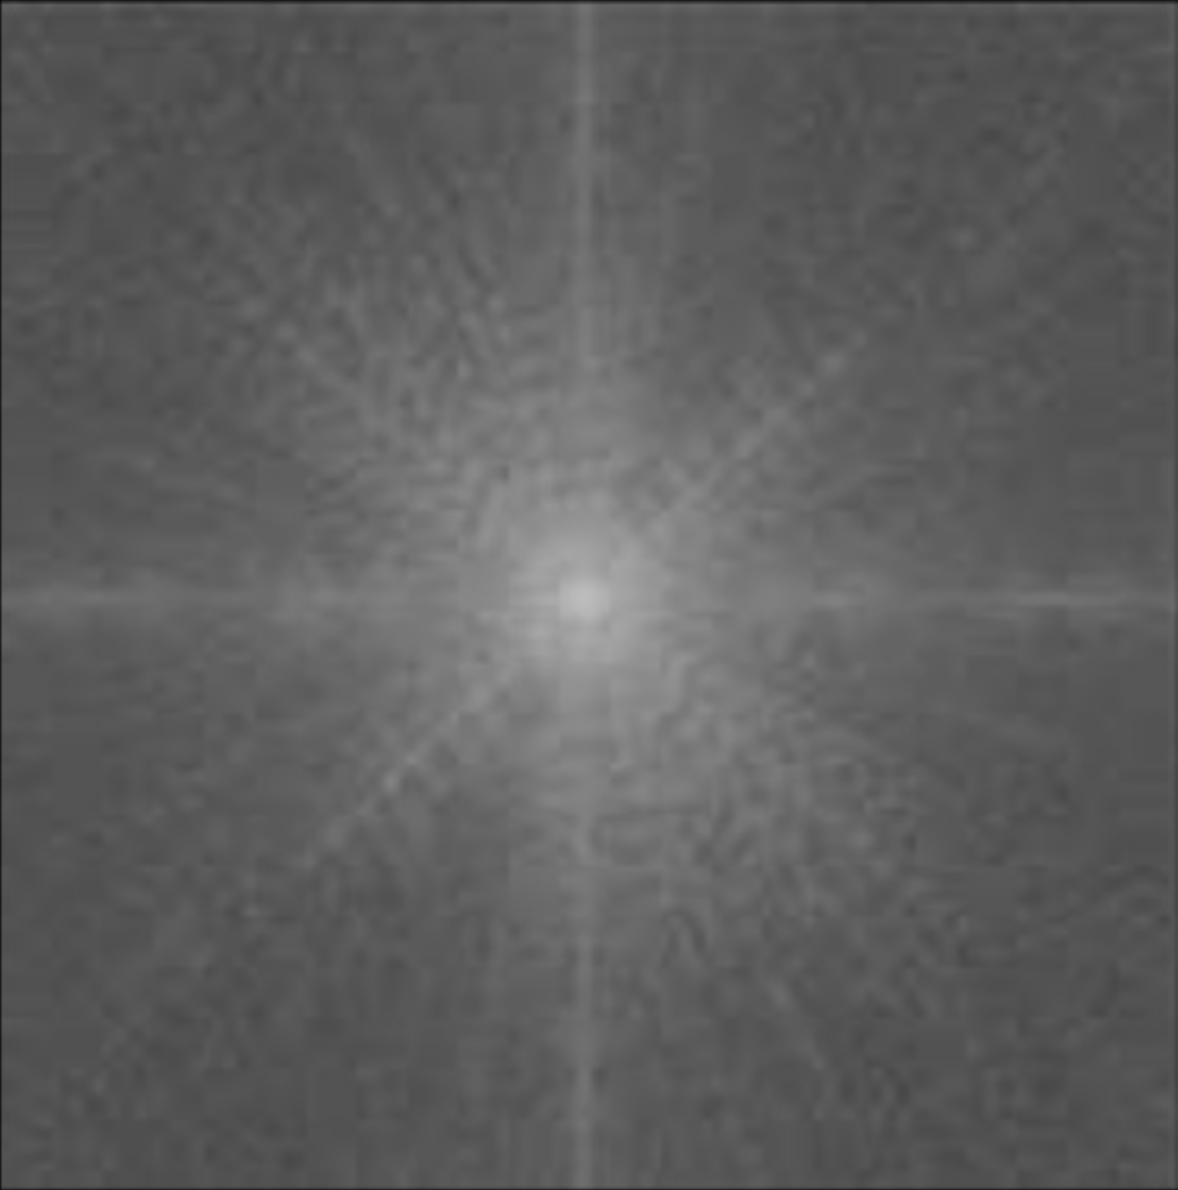
\includegraphics[width=.8\textwidth]{K_space}\\
                \column{.5\textwidth} \centering
                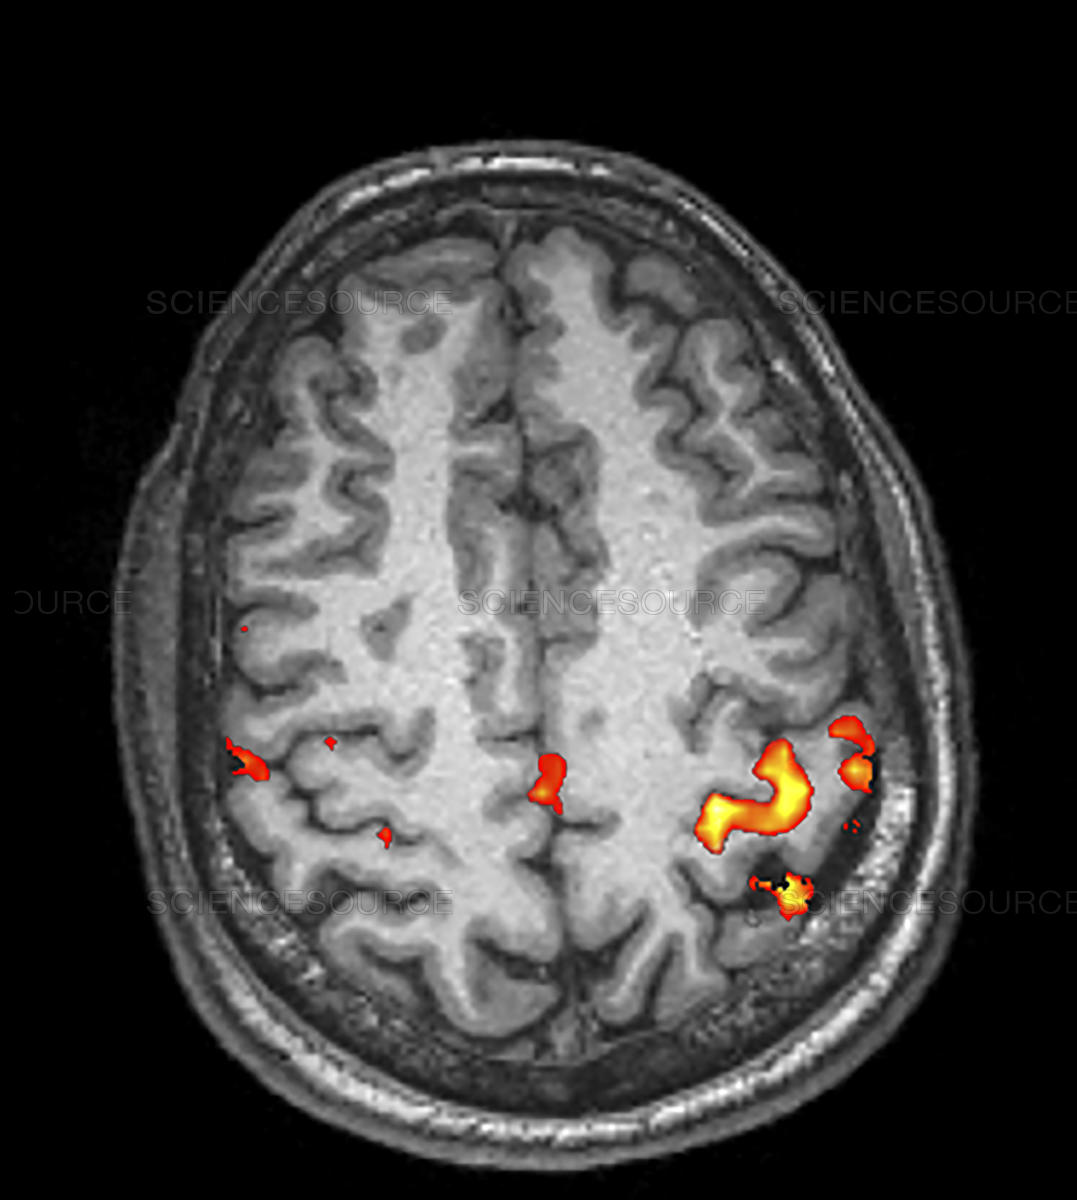
\includegraphics[width=.8\textwidth]{brain_scan}\\
                \end{columns}

            \vskip1.5em
            {\bf Imaging}\\[1em]
            \centering
            \uncovergraphics<1>[width=.8\textwidth, trim={0em 2em 37em 2em}, clip]{super_resolution.png}\\
            Super-Resolution, Inpainting, Deblurring, ...
        \end{columns}

        \vskip-13em
        {\centering\highlight{
            \parbox{.7\textwidth}{
                \vskip1em\centering
                For many inverse problems, we don't have access to
                large training sets with pairs $(\varX, \varZ)$.
                \vskip1em
            }
        }\\}

}


\frame[t]{
    \frametitle{Inverse Problem Resolution}
    {\bf Regularized regression problem}\\[.5em]

    \alt<-2>{\[
        f(\varX) = \argmin_\varZ \frac12\|\varX - \varD\varZ\|_2^2 + \mathcal R(\varZ{})
    \]}{\[
        f(\varX) = \argmin_\varZ \frac12\|\varX - \varD\Phi_\Theta(\varX)\|_2^2 + \mathcal R(\Phi_\Theta(\varX))
    \]}
    where $\mathcal R$ encodes prior information to select a good/plausible solution.\\[1em]

    \only<2>{
        \begin{columns}[T]
            \column{.47\textwidth}
            \underline{Classical regularization:}\\[1em]
            \begin{itemize}\itemsep.5em
                \item Norms:
                    $\ell_2, \ell_1$, TV,\\
                    \mycite{Hamalainen1984}
                \item Dictionary:
                    Wavelets, Time-Freq.\\
                    \mycite{Gramfort2012}
            \end{itemize}
            \column{.47\textwidth}
            \underline{Data-driven regularization:}\\[1em]
            \begin{itemize}\itemsep.5em
                \item Dictionary-learning,\\
                \mycite{Olshausen1997}
                \item Plug-and-Play methods.\\
                \mycite{Venkatakrishnan2013}
            \end{itemize}
        \end{columns}
    }
    \only<3->{%
        \underline{Parametric form for $\varZ = \Phi_\Theta(\varX)$}\\[1em]

        \begin{itemize}\itemsep.5em
            \item  Domain specific solutions:\\
            \hskip2ex \emph{Dipole Fit.} \mycite{Sarvas1987}
            \item{} Deep-learning based:\\
            \hskip2ex \emph{Deep Image Prior, Algorithm unrolling.} \mycite{Ulyanov2020}
        \end{itemize}
    }
    \only<4>{
        \vskip1em
        {\bf Algorithm unrolling:}
        Design $\Phi_\Theta$ based on a solver for a regularized inverse problem.
    }
}

% \frame{
%     \frametitle{Machine Learning approach}

%     {\bf Using deep learning to solve inverse problem:}\\[1em]
%     Learn a neural network $\Phi_\Theta$ that maps $\varX$ to $\varZ$.


%     \vskip1em
%     \begin{columns}
%         \column{.42\textwidth}
%         \highlight{\parbox{\textwidth}{
%             {\bf Supervised}\\[.5em]\color{black}\normalsize\normalfont
%             Access to the ground truth $\varZ$:
%             \[
%                 \min_\Theta \mathbb E_{\varX,\varZ}\Big[\frac12\|\varZ - \Phi_\Theta(\varX) \|_2^2\Big]
%             \]
%             \phantom{$\mathcal R$g}
%         }}
%         % \column{.005\textwidth}
%         \column{.52\textwidth}
%         \highlight{\parbox{\textwidth}{
%         {\bf Unsupervised}\\[.5em]\color{black}\normalsize\normalfont
%         No ground truth:
%         \[
%             \min_\Theta\mathbb E_{\varX}\Big[\frac12\|\varX - \varD\Phi_\Theta(\varX) \|_2^2 \Big]
%         \]
%         Can regularize the output with $\mathcal R$.
%         }}

%     \end{columns}

%     \vskip2em
%     {\bf Algorithm unrolling:}\\[1em]
%     Design $\Phi_\Theta$ based on a solver for a regularized inverse problem.
% }

\begin{frame}{Algorithm unrolling for Sparse Inverse Problem}

    {\centering
    \begin{tikzpicture}
    \tikzset{
        %Define standard arrow tip
        >=stealth',
        %Define style for boxes
        varstyle/.style={
            rectangle,
            rounded corners,
            draw=black,
            text width=1em,
            minimum height=1.5em,
            text centered},
    }
    \node (meg) {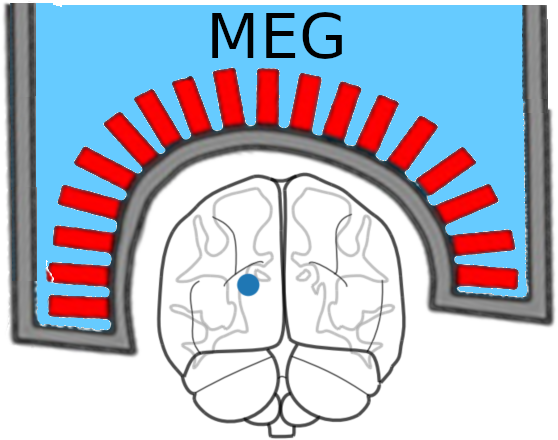
\includegraphics[width=8em]{meg_localised_source_point}};
    \draw[->, thick] ($(meg.east) - (0, 1em)$) -- ++(8em, 0)
    node[midway, align=center] (maxwell) {Maxwell's\\Equations}
    node[right] (topomap) {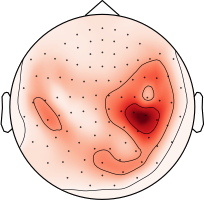
\includegraphics[width=4em]{topomap_somato}};
    \node[varstyle, below=.5em] at (topomap.south) (varX) {$\varX$};
    \node[below=0em of varX.south] {\bf Observed signal};
%        \draw[->, thick] (topomap.east) -- ++(5em, 0)
%        node[midway, align=center] {\small Problème\\ \small inverse}
    \node[varstyle, below=.2em of meg]
        (varZ) {$\varZ$};
        \node[below=0em of varZ.south] {\bf Electrical activity};
    \node[varstyle, below=2.9em of maxwell.center]
        (varD) {$\varD$};

    \draw[<-, thick] (meg.east) to[bend left, looseness=1]
    node [midway, above] {Inverse Problem}
    ($(topomap.west) + (0, 1em)$);
    \end{tikzpicture}\\[1em]}

    For $\lambda > 0$, the sparse inverse problem solution is \\[.5em]
    \[
        z^{*} = \argmin_{\varZ} F_\varX(\varZ) =
        \underbrace{\frac{1}{2}\| \varX - \varD \varZ\|_2^2}_{f_\varX(\varZ)}
        + \lambda\| \varZ\|_1
    \]
    \emph{a.k.a.} Lasso, sparse linear regression, sparse coding...\\[1em]
    % We are interested in the case where $m > n~.$\\[2em]
    % {\centering
    % \setlength\bodywd{.9\linewidth}
    % \begin{block}{\bf Properties}
    %     \begin{itemize}\color{black}\itemsep.5em
    %         \item The problem is convex in $z$ but not strongly convex in general
    %         \item $z=0$ is solution if and only if
    %             $\lambda \ge \lambda_{\max} \doteq \|G^\top x\|_\infty$
    %     \end{itemize}
    % \end{block}}
\end{frame}

\begin{frame}[t]{Iterative Shrinkage-Thresholding Algorithm \mycite{Daubechies2004}}
    Proximal gradient descent algorithm
    \alt<1>{\[
        z^{(t+1)} = st\left(z^{(t)}
                                   - \frac{1}{L}\underbrace{\nabla f_x(z^{(t)})}_{G^\top(G z^{(t)} - x)},
                                   \frac{\lambda}{L}\right)
    \]}{\[
        z^{(t+1)} = st\left(
            \textcolor{linkcolor}{(Id - \frac{1}{L}G^\top G)} z^{(t)}
            + \textcolor{D}{\frac1LG^\top} x,
            \textcolor{Z}{\frac{\lambda}{L}}
        \right)
    \]}
    where $L = \|G^\top G\|_2$ is the largest eigenvalue of $G^\top G$.\\
    Here, $1/L$ plays the role of a step size.\\[1em]

    \only<1>{
        \begin{columns}[T]
            \column{.48\textwidth}

            $st$ is the soft-thresholding operator.\\[2em]
            \myitem{} Proximal operator for $\ell_1$-norm.\\[1em]
            \myitem{} Push for sparse vector.
            \column{.5\textwidth}
            \vskip-1em
            \centering
                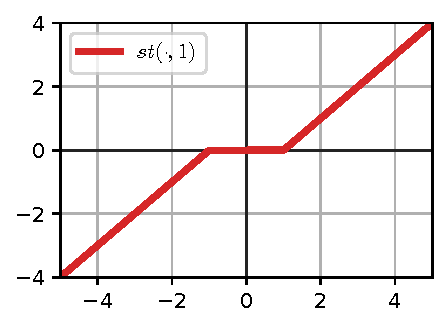
\includegraphics[width=.8\textwidth]{soft_thresholding}\\
        \end{columns}
    }
    \only<2->{
        \begin{columns}
            \column{.55\textwidth}
                {\bf Computational graph interpretation:}\\[1em]
                \myitem{} $W_z = \textcolor{linkcolor}{Id - \frac1{L}G^\top G}$\\[.5em]
                \myitem{} $W_X = \textcolor{D}{\frac1{L}G^\top} $
                \hskip2ex\myitem{} $\beta=\textcolor{Z}{\frac{\lambda}{L}}$
            \column{.45\textwidth}
            \vskip2em
            \inputTikZ{.8}{one_step_ista.tex}
        \end{columns}
    }
\end{frame}

\frame[t]{
    \frametitle{Learned ISTA \mycite{Gregor2010}}

    {\bf \alt<2->{Learned}{Unrolled} ISTA:\\[1em]}
    {\centering\alt<2->{
        \inputTikZ{.8}{lista_tikz.tex}
    }{
        \inputTikZ{.8}{ista_unrolled}
    }\\[1em]}

    \alt<2->{
        Learn the weights
        $\Theta = (W_X^{(t)}, W_z^{(t)}, \beta^{(t)})_{t=0}^T$\\[1em]
    }{
        Equivalent to ISTA with $W_z = Id - \frac{1}{L}G^\top G$, $W_X = \frac{1}{L}G^\top $ and $\beta = \frac\lambda{L}$.\\[1em]

        \only<1>{\centering 3 iterations of ISTA $\Leftrightarrow$ 3 layers in the neural network\\}
    }

    % \only<2>{
    %     \vskip2em
    %     If the number of layer goes to infinity, ISTA is equivalent to the RNN:\\[1em]
    %     \begin{columns}
    %         \column{.5\textwidth}
    %         {\centering\inputTikZ{.8}{ista_tikz.tex}\\}
    %         \column{.5\textwidth}
    %         {\bf Implicit deep learning (DEQs):\\[.5em]}
    %         $z^* = st(W_z z^* + W_X x, \beta)$
    %     \end{columns}
    % }

    \only<2-3>{

        \begin{columns}[T]
            \column{.42\textwidth}
                \uncover<-2>{
                \highlight{\parbox{\textwidth}{
                    {\bf Supervised}\\[.5em]\color{black}\normalsize\normalfont
                    Access to the ground truth $z$:
                    \[
                        \min_\Theta\mathbb E_{x,z}\Big[\frac12\|z - \Phi_\Theta(x) \|_2^2\Big]
                    \]
                }}}
                \only<3>{\vskip-7em \centering\highlight{
                    \parbox{.85\textwidth}{
                        Many works for images\\[.5em]
                        \footnotesize\normalfont \color{black}
                        see review \citep{Monga2021}
                    }
                }}

            \column{.52\textwidth}

            \highlight{\parbox{\textwidth}{
            {\bf Unsupervised}\\[.5em]\color{black}\normalsize\normalfont
            No ground truth:
            \[
                \min_\Theta\mathbb E_{x}\Big[\frac12\|x - G\Phi_\Theta(x) \|_2^2 + \lambda \|\Phi_\Theta(x)\|_1\Big]
            \]
            }}
        \end{columns}
    }

}

\frame{
    \frametitle{}


    \highlightbox{
        \bf Learning to optimize with unrolled ISTA\\[.5em]
        \color{black}\normalfont
        \myitem{} Can LISTA go faster than ISTA?\contrib{Moreau and Bruna, ICLR 2017}\\
        \myitem{} What does LISTA learn?\contrib{Ablin et al., NeurIPS 2019}\\[.5em]
    }
    \vskip2em
    \highlightbox{
        \bf Learning the regularizer $\mathcal R$ from data\\[1em]
        \color{black}\normalfont
        \myitem{} How to leverage unrolled algorithms to learn $\mathcal R$?\\
        \myitem{} How does it compare with classical algorithm?\\
        \contrib{Malézieux et al., ICLR 2022}\\[.5em]
    }

}

\section{Learning to optimize with unrolled ISTA}
\parttitleframe{Moreau2017,Ablin2019}


\frame{
    \frametitle{Solving many inverse problems}


    \hskip-.7ex{\bf Context:} Many inverse problems with the same structure $G$.\\[1em]
    \myitem{} One per time sample for MEG: $> 50k$ instances.\\[1em]
    \begin{columns}[c]

        \column{.55\textwidth}

        {\bf Goal:} learn $\Phi_\Theta$ with $T$ layers such that:
        \[
            F_x(\Phi_\Theta(x)) < F_x(ISTA_T(x))
        \]

        {\bf Questions:}\\[1em]
        \myitem{} How fast can LISTA go?\\[.5em]
        \myitem{} What does LISTA learn?\\[1em]

        \column{.45\textwidth}
        {\centering
        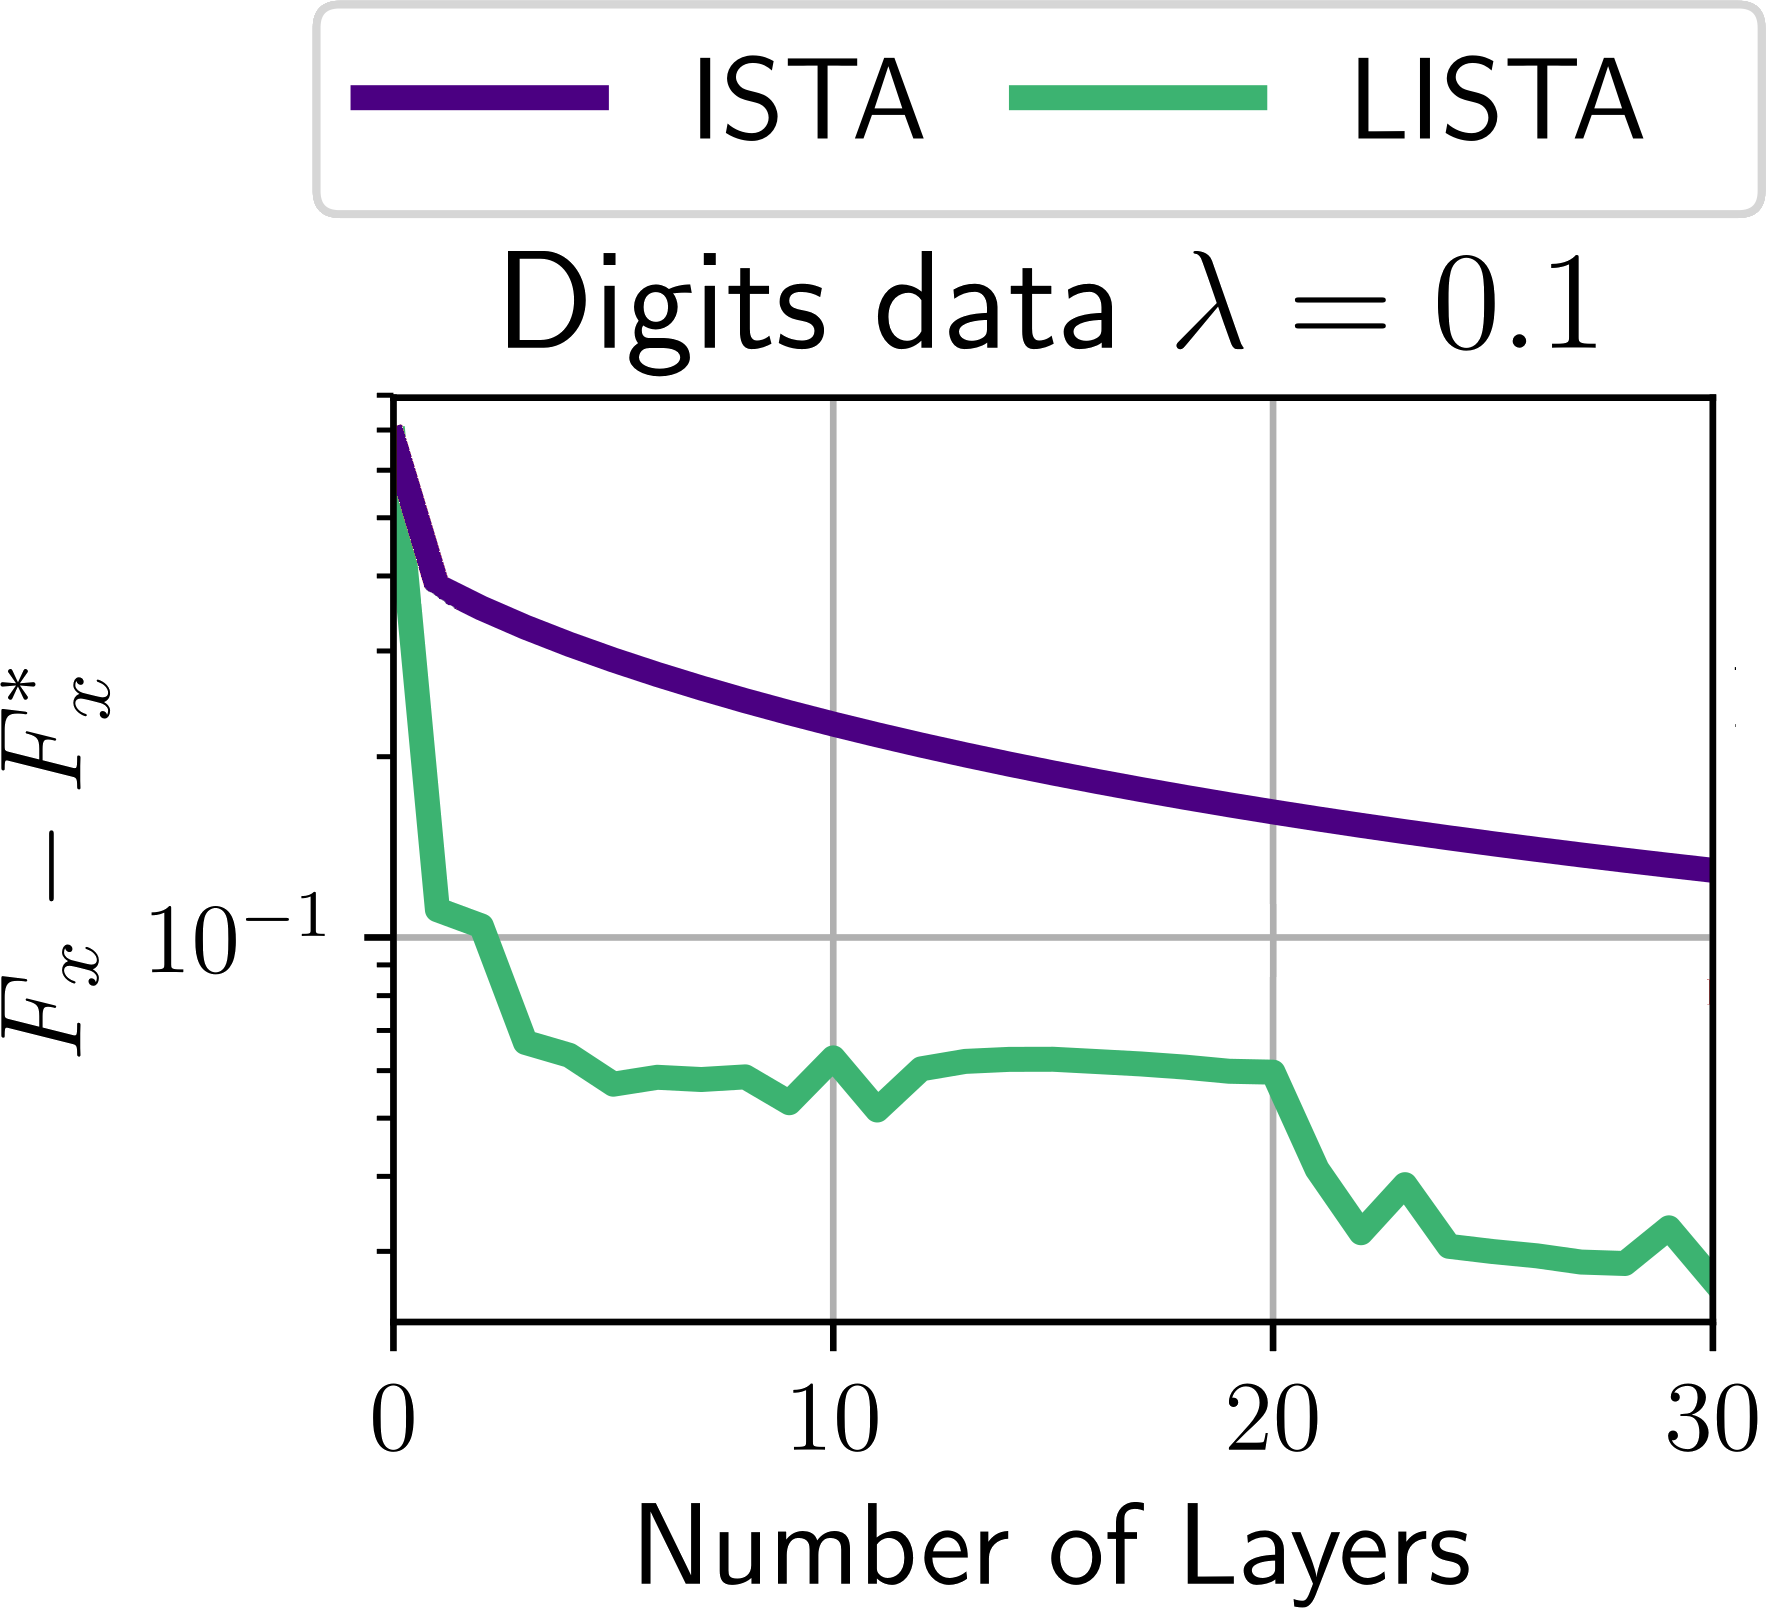
\includegraphics[width=\textwidth]{comparison_lista.png}\\}
    \end{columns}
}

\frame{
    \frametitle{How fast can LISTA go? \contrib{Moreau and Bruna, 2017}}

    Results are based on a quasi-diagonalization $G^\top G \simeq V^\top \Lambda V$ that does not distort ``too much'' the $\ell_1$-norm.\\[2em]

    \myitem{} For a class of parameters, LISTA has the same cvg rate as ISTA.\\[1em]
    \myitem{} LISTA can benefit from improved constants.\\[1em]
    \myitem{} As the optimization approaches a solution, it is harder and harder to get improved constants.\\[2em]


    \strongpoint{Shows that it is possible to improve the first iterations of the algorithm.}
}

\frame{
    \frametitle{What does LISTA learn? \contrib{Ablin et al., 2019}}

    Consider that the number of layers goes to $+\infty$.\\[1em]
    \begin{block}{Theorem -- Asymptotic convergence of the weights}
        Assume that the weights of the network converge to a limit:
        \[
            W_z^{(t)}, W_X^{(t)}, \beta^{(t)} \to W_z^*, W_X^*, \beta^*
            \qquad as \qquad t\to +\infty
        \]
        and that the output of the network converges to a solution of the unsupervised problem.\\[.5em]
        Then
        \[
            W_z^* = Id - \alpha D^\top D, \quad
            W_X^* = \alpha D^\top, \quad
            \beta^* = \alpha \lambda, \quad
        \]
    \end{block}

    \strongpoint{Correspond to ISTA with step size $\alpha$ instead of $\frac1L$}
}


\frame{
    \frametitle{Intuition for the result}

    The network's output $\Phi(x)$ for all input $x$ needs to verify:
    \begin{align*}
        \Phi(x) = & ~ st\big(
            \textcolor{linkcolor}{(Id - \frac1L G^\top G)}\Phi(x)
            + \textcolor{D}{\frac1L G^\top} x,
            \textcolor{Z}{\frac\lambda{L}}
        \big) \qquad\qquad\keypoint{\text{KKT}}\\[.5em]
        \Phi(x) = &~st\big(
            \textcolor{linkcolor}{W_z^*}\Phi(x)
            + \textcolor{D}{W_X^*} x,
            \textcolor{Z}{\beta^*}
        \big) \qquad\qquad\quad\keypoint{\text{Weights cvg}}
    \end{align*}
    \vskip2em
    \myitem{} If verified uniformly, this imposes a strong structure on the asymptotic weights.\\[1em]
    \myitem{} This structure can be relaxed based on the distribution of $x$.
}

% \begin{frame}{Numerical verification}
%     \centering
%     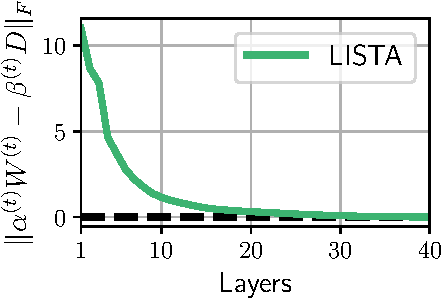
\includegraphics[width=.8\textwidth]{fro_similarity}\\[1em]
%     40-layers LISTA network trained on a $10 \times 20$ problem with $\lambda = 0.1$\\
%     {\bf The weights $W^{(t)}$ align with $D$ and $\alpha, \beta$ get coupled.}


% \end{frame}


\begin{frame}{Step LISTA \contrib{Ablin et al., 2019}}

    Inspired by this result: learn adapted step sizes for ISTA.\\[2em]
    {\bf Restricted parametrization :}
    Only learn a step-size $\alpha^{(t)}$\\[1em]
    \[
    z^{(t+1)} = \text{ST}\left(z^{(t)}
              - \textcolor{linkcolor}{\bf\alpha^{(t)}} D^\top(D z^{(t)} -x),
              \lambda\textcolor{linkcolor}{\bf\alpha^{(t)}}\right)
    \]
    \vskip1em
    \underline{Fewer parameters:}\\[1em]
    % $T$ instead of $( 2 + mn)T~.$\\[1em]
    \begin{columns}[c]
        \column{.5\textwidth}
            \myitem{} Easier to learn\\
        \column{.5\textwidth}
            \myitem{} Fewer degrees of freedom\\
    \end{columns}
    \vskip2em
    \centering $\Rightarrow$ Reduced performances?\\

\end{frame}




% \begin{frame}[t]{Performances}

%     {\bf Simulated data:} $m=256$ and $n=64$\\[.7em]
%     \hskip6ex $D_k \sim \mathcal U(\mathcal S^{n-1})$ and $x = \frac{\widetilde x}{\|D^\top \widetilde x\|_\infty}$ with $\widetilde x_i \sim \mathcal N(0, 1)$\\[1.5em]
%     {\centering
%     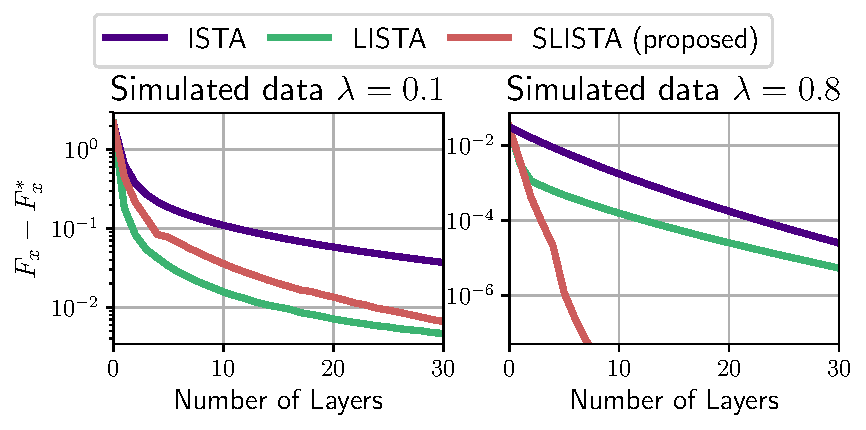
\includegraphics[width=\textwidth]{comparison_networks_simu}\\}
% \end{frame}

\begin{frame}{Performance of SLISTA}

    {\bf Digits:} $8\times 8$ images \mycite{Pedregosa2011}\\[.7em]
    \hskip6ex $G_k $ and $\widetilde x$ sampled uniformly from the digits and $x = \frac{\widetilde x}{\|G^\top \widetilde x\|_\infty}$.\\[1.5em]
    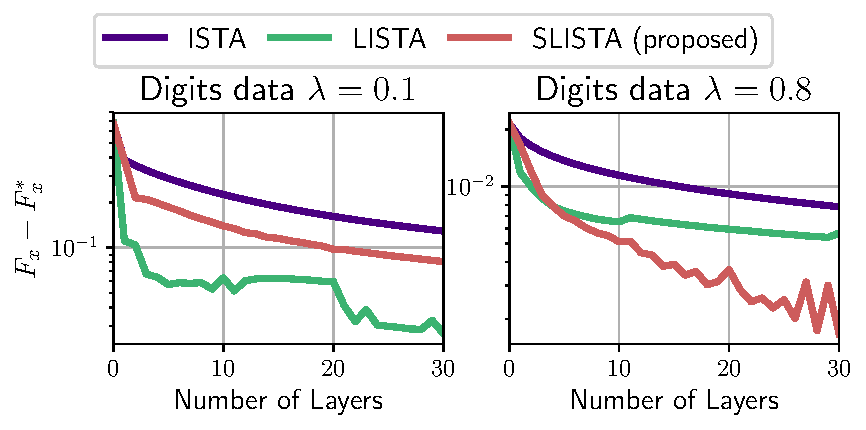
\includegraphics[width=\textwidth]{comparison_networks_images}

\end{frame}

\begin{frame}{Learning better step sizes}
    Linked to better step-sizes for ISTA in $\big[\frac1{L_S}, \frac2{L_S}\big[$ when $Supp(z^{(t)}) = S$\\[.5em]
    $L_S$ is the largest eigenvalue of $G^\top G$ restricted on the support $S$\[
        \max_{\substack{Supp(z) = S\\\|z\|_2\le 1}} z G^\top G z
    \]
    \centering
    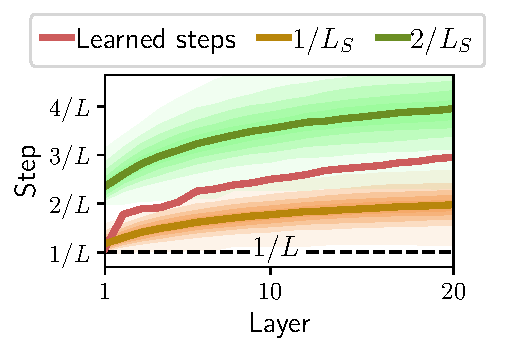
\includegraphics[width=.6\textwidth]{learned_steps}\\
    % The learned step-sizes are linked to the distribution of $1/L_S$\\[1em]


\end{frame}


\frame{
    \frametitle{Unrolling for learned optimization}

    \vskip4em
    {\centering\bf No hope to learn an algorithm that converges\\faster than ISTA \underline{uniformly}.\\[2em]}

    \begin{itemize}\itemsep.5em
        \item But one can learn parameters (step-size) of the algorithm that better adapt to the input distribution.\\
        \contrib{Ablin et al., 2019}
        \item Also possible to improve the first iterations of ISTA (improve constants).\\
        \contrib{Moreau and Bruna, 2017}
    \end{itemize}

    \vspace{0pt plus 1 filll}
    \footnotesize
    Also considered unrolled algorithms for TV in  Cherkaoui, Sulam, {\bf M.}, NeurIPS 2020.

}



\section{Learning $\mathcal R$ with unrolled algorithm}
\parttitleframe{Malezieux2022}

\frame[t]{
    \frametitle{Prior Learning}

    {\bf Inverse Problem Prior:} choosing $\mathcal R$.\\[1em]

    \underline{Typical prior:} Signal $z$ is sparse in a specific dictionary $D$.\\[2em]

    \begin{columns}[T]
        \column{.49\textwidth}
        \uncover<-2>{
            \textbf{Analysis formulation:}\\$\varZ$ is sparse in $D$.
            \[
                \min_u\frac12\|\varX-\varD\varZ\|_2^2 + \lambda\|D^T\varZ\|_1 \enspace .
            \]
        }
        \column{.49\textwidth}
        \textbf{Synthesis formulation:}\\$u$ sparse to synthesize $\varZ = Du$.
        \[
            \min_u\frac12\|\varX-\varD Du\|_2 + \lambda\|u\|_1 \enspace .
        \]
    \end{columns}


    \vskip1em
    \only<2>{
        {\bf Fixed dictionaries:}\\[.5em]
        \myitem{} Total-variation for signals and images. \mycite{Rudin1992}\\
        \myitem{} Wavelets for images. \mycite{Mallat2008}\\
        \myitem{} Time-frequency atoms for MEG.\mycite{Gramfort2012}\\[2em]
    }
    \only<3>{
        {\bf Data driven dictionary:}  Learn $D$ from the data $\varX$.
        % \[
        %     \min_{\substack{D,u\\ \|D_k\|_2 \le 1}} F(D, u) \triangleq \frac12\|x - GDu\|_2^2 + \lambda\|u\|_1
        % \]
    }
}

\frame{
    \frametitle{Dictionary Learning \mycite{Olshausen1997}}
    Solve the following non-convex problem:
    \[
        \min_{\substack{D,u\\ \|D_k\|_2 \le 1}} F(D, u) \triangleq \sum_{i=1}^N\frac12\|x^i - GDu^i\|_2^2 + \lambda\|u^i\|_1
    \]

    \vskip2em
    \underline{Classical algorithm:} Alternate Minimization (AM)\\[1em]

    \myitem{} Minimize $F(D, \cdot)$ in $u$ with $T$ iterations of ISTA with fixed $D$:
    \[
        u_T = ISTA_T(x)
    \]
    \myitem{} Minimize $F(\cdot, u_T)$ in $D$ with projected gradient descent:\\
    \[
        g^1_T(D) = \nabla_1 F(D, u_T)
    \]
}

\frame[t]{
    \frametitle{Unrolling for dictionary learning}

    \setbeamercovered{invisible}

    {\bf Bi-level formulation:}
    \[
        \min_{\substack{\|D_k\|\le 1}} h(D) \triangleq F(D, u^*(D))
        \quad s.t. \quad
        u^*(D) = \argmin_u F(D, u)
        \enspace.
    \]
    Optimization problem in $D$ solved with projected gradient descent.\\
    \strongpoint{
        How to estimate the gradient $g^*(D) = \nabla h(D)$ efficiently?
    }\vskip1em

    \only<2-3>{

        {\bf Danskin Theorem:} \mycite{Danskin1967}
        \[
           g^*(D) = \nabla_1 F(D, u^*(D))
        \]
        \emph{This is due to the fact that ``~$\nabla_2 F(D, u^*(D)) = 0$''.}\\[2em]

        \visible<3>{{\bf Issue:} computing $u^*(D)$ is computationally expansive.}
    }
    % \only<4>{
    %     \textbf{Alternate Minimization:}\\[.5em]
    %     Replace $u^*(D)$ by $u_T(D)$ in the expression of $g^*$:
    %     \[
    %         g^1_T(D) = \nabla_1 F(D, u_T(D))
    %     \]
    %     \vskip1em
    %     Does not account that moving $D$ will also move $u_T(D)$.
    % }
}

\frame[t]{
    \frametitle{Unrolling for dictionary learning}
        \textbf{Unrolled formulation:}\\[.5em]
    \[
        \min_{\substack{\|D_k\|\le 1}} h_T(D) \triangleq F(D, u_T(D))
        \enspace.
    \]
    The gradient estimate becomes:
    \[
        g^2_T(D) = \nabla_1 F(D, u_T(D)) + J_T^\top\nabla_2 F(D, u_T(D))
    \]
    Estimate the jacobian $J_T = \frac{\partial u_T}{\partial D}$ with back-propagation.
    % \vskip1em
    % \begin{columns}
    %     \column{.39\textwidth}
    %         \underline{Re-parametrization:}\\[.5em]
    %         \myitem{} $W_X = \frac{D^\top G^\top}{L} $\\
    %         \myitem{} $W_z = Id - \frac{D^\top G^\top GD}{L}$
    %     \column{.59\textwidth}
    %         {\centering\inputTikZ{.5}{ista_unrolled}\\[1em]}
    % \end{columns}
    \only<2>{
        \vskip1em
        {\centering
        \highlight{
            {\bf Question:} Is it more efficient to use unrolling or AM?
        }}

        \vskip2em
        \myitem{} Work for smooth problems.\contrib{Ablin et al., ICML 2020}\\[1em]
        \myitem{} Improved performances for supervised learning.\mycite{Monga2021}\\
    }


}


\frame[t]{
    \frametitle{Gradient Estimation \contrib{Malézieux et al., 2022}}

    \begin{columns}[T]
        \column{.45\textwidth}
        {\bf Alternate Minimization}\\[.5em]
        No Jacobian estimation
        \[
            g^1_T(D) = \nabla_1 F(D, u_T(D))
        \]
        \column{.02\textwidth}
            \rule{.1mm}{.33\textheight}
        \column{.48\textwidth}
        {\bf Unrolled ISTA}\\[.5em]
        Account for Jacobian of $u_T$
        \[
            \begin{split}
                g^2_T(D) = & \nabla_1 F(D, u_T(D))\\
                   & + J_T^\top\nabla_2 F(D, u_T(D))
            \end{split}
        \]
    \end{columns}

    \vskip1.5em
        \begin{columns}[T]
            \column{.45\textwidth}
            \only<2->{
                Converges as fast as $u_T$
                \[
                    \|g^1_T - g^*\|_2 \le L_1 \|u_T - u^*\|_2
                \]
            }
            \column{.02\textwidth}
                \vskip-4em\rule{.1mm}{.52\textheight}
            \column{.48\textwidth}

            \only<3->{
                May converge faster than $u_T$
                \[
                    \begin{split}
                        \|g^2_T - g^*\| \le & L\|J_T-J^*\|_2\|u_T - u^*\|_2\\
                                            & + L_2\|u_T - u^*\|_2^2
                    \end{split}
                \]
                \strongpoint{Need to study $\|J_T - J^*\|_2$.}
            }
        \end{columns}
        \vskip2em


        \only<4->{\footnotesize
        Similar results for smooth function in \emph{Ablin, Peyré, {\bf M.} ICML 2020}.}
}

\frame{
    \frametitle{Jacobian Estimation \contrib{Malézieux et al., 2022}}

    \begin{tcolorbox}[title=\textbf{Convergence of the Jacobian}]
        \[
        \|J_T - J^*\|_2 \le A_T + B_T \enspace .
        \]
        $A_T$ converges linearly towards 0, $B_T$ is an error term which may increase for large $T$ and vanishes on the support of $u^*$.
    \end{tcolorbox}

    \vskip2em
    \myitem{} On the support, the jacobian converges linearly.\\[1em]
    \myitem{} Before reaching the support, $B_T$ is an error term that can accumulate.\\[1em]
    \myitem{} \parbox[t]{.8\textwidth}{
        $B_T$ can be attenuated with truncated back-propagation.
    }
}

\frame{
    \frametitle{Empirical evaluation}

    {\centering
    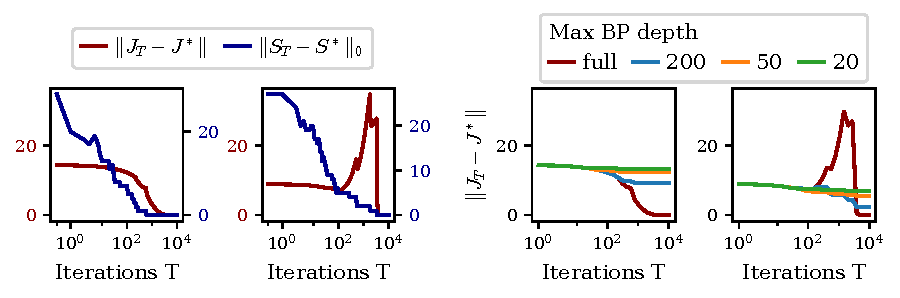
\includegraphics[width=.7\linewidth,trim={0 0 20em 0}, clip]{conv_jac.pdf}\\[1em]}

    \myitem{} Linear convergence once the support $S^*$ is reached.\\[1em]
    \myitem{} Possible explosion before reaching $S^*$.

}

\frame{
    \frametitle{Empirical evaluation}

    {\centering
    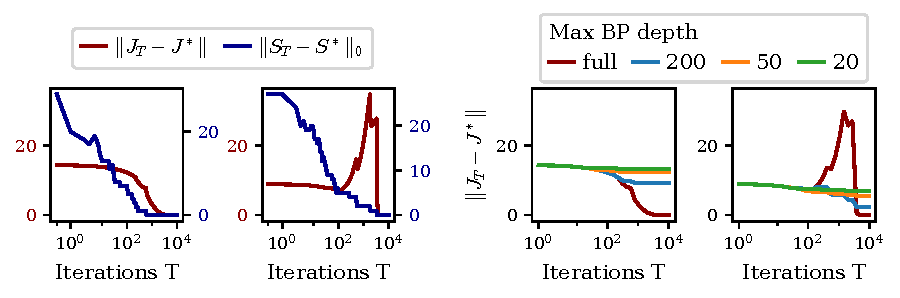
\includegraphics[width=.7\linewidth,trim={20em 0 0 0}, clip]{conv_jac.pdf}\\[1em]}

    \myitem{} Truncated backpropagation (BP) reduces the explosion.\\[1em]
    \myitem{} Less precise when the support is reached.

}



\frame{
    \frametitle{Numerical experiments on gradient}

    {\centering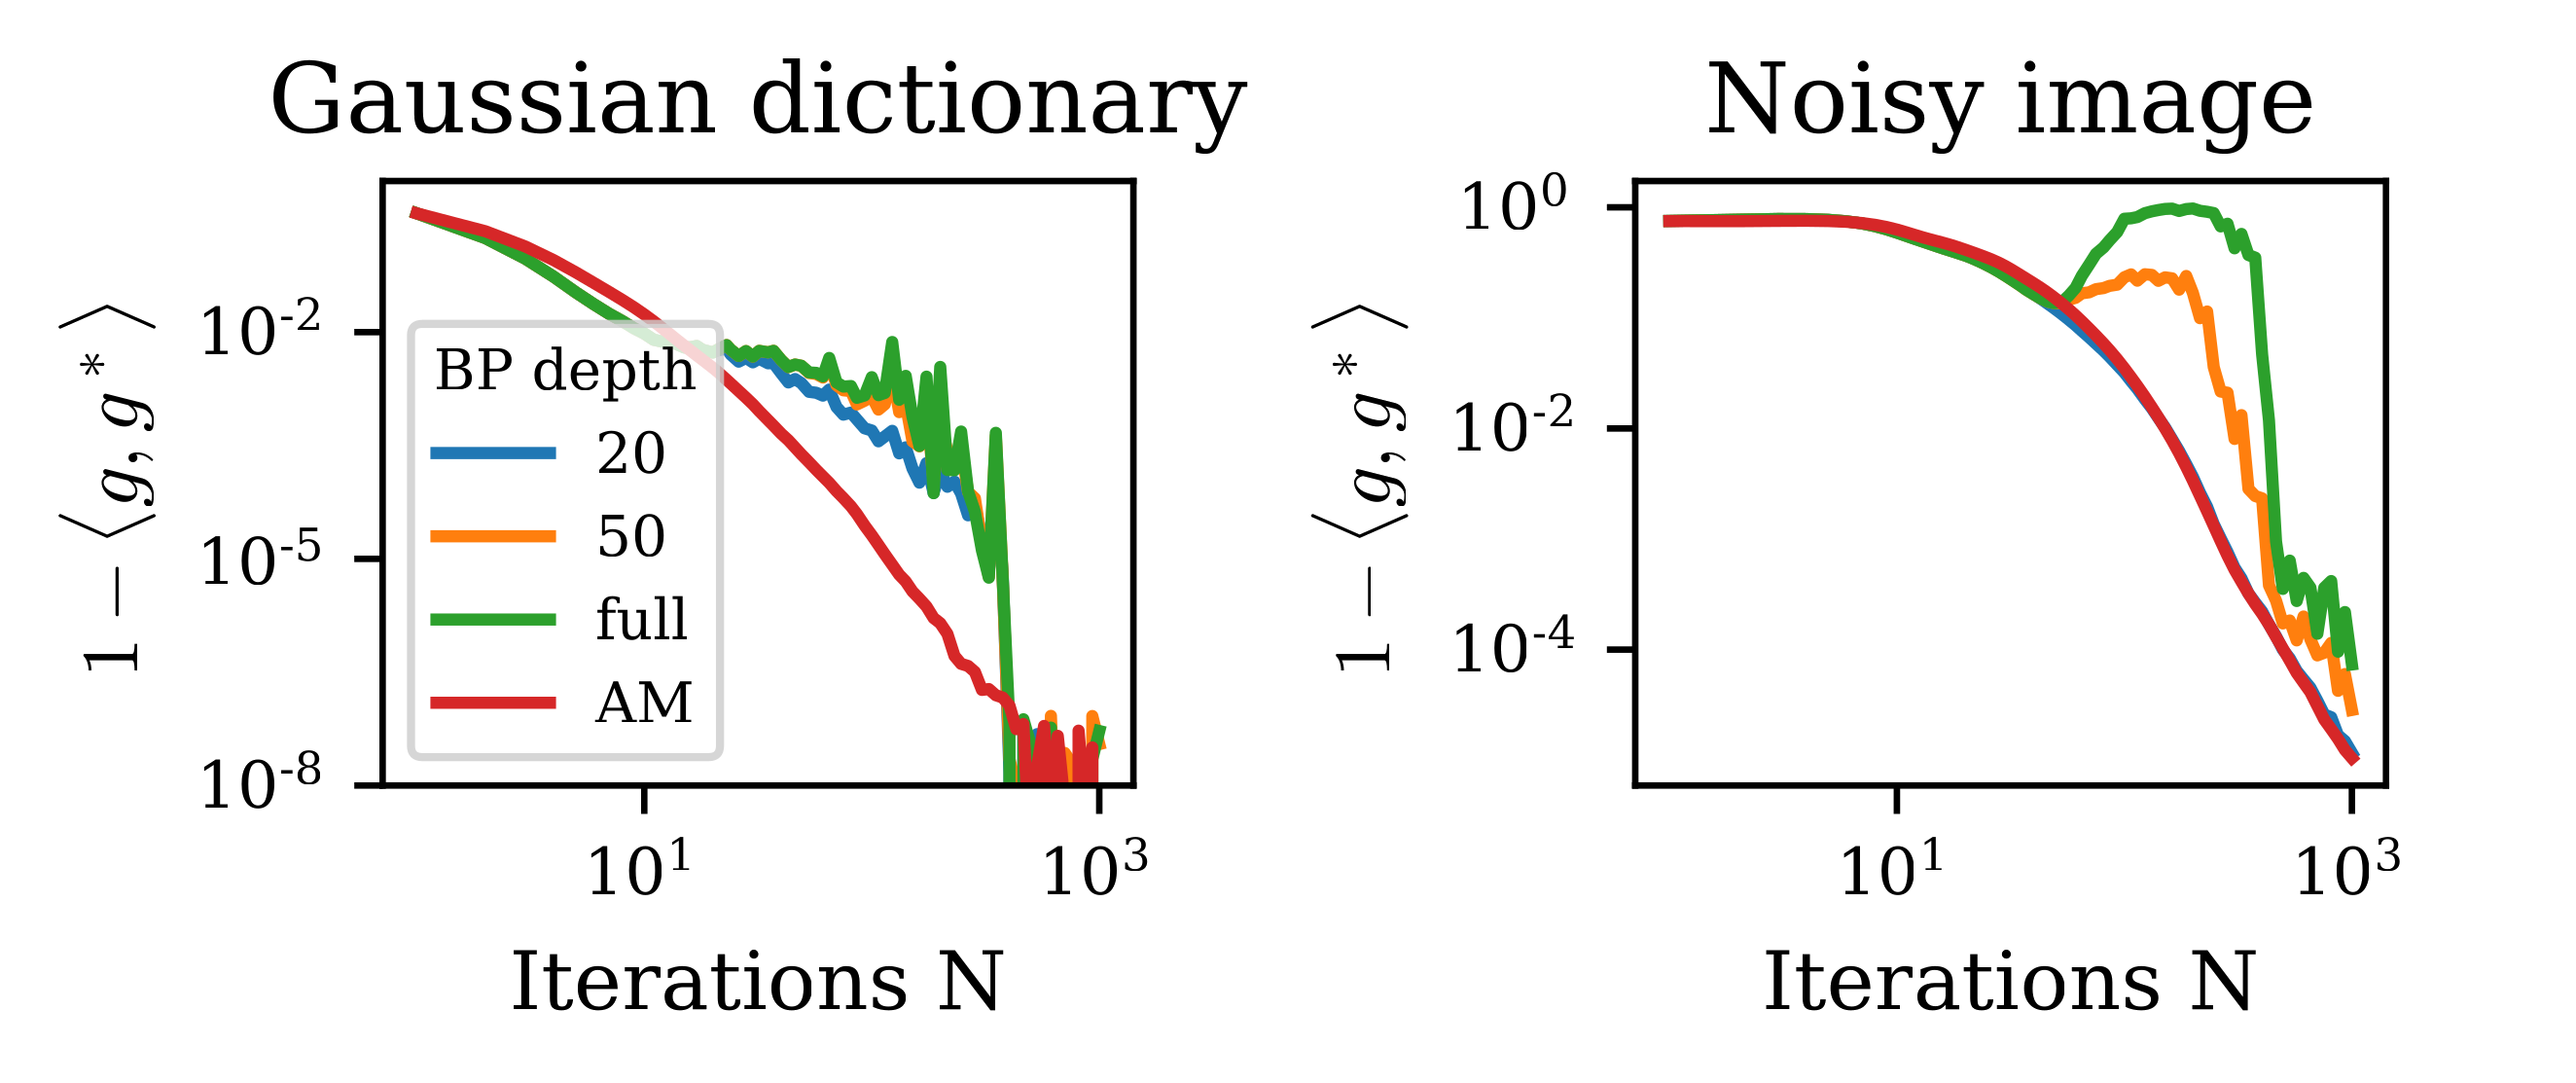
\includegraphics[width=.8\linewidth]{gradients_small.png}\\[1em]}
    \myitem{}\textbf{First iterations:} Stable behavior.\\[1em]
    \myitem{}\textbf{Too many iterations:}
        Numerical instabilities due to the accumulation of errors.
        Truncated back-propagation reduces the errors.\\[1em]
    \myitem{}\textbf{On the support:} Convergence towards $g^*$.
    \vskip1em
}

\frame{
    \frametitle{Impact on Dictionary Learning}

    \setbeamercovered{invisible}

    \begin{columns}
        \column{.55\textwidth}
        Comparison of 3 schemes to learn dictionaries on generated data:\\[1em]
        \begin{itemize}\itemsep.5em
            \item {\bf AM:} use gradient estimate $g^1_T$
            \item {\bf DDL:} use gradient estimate $g^2_T$
            \item {\bf DDL+step:} DDL + learn the step\\size in the unrolled algorithm $u_T$.
        \end{itemize}
        \column{.45\textwidth}
        {\centering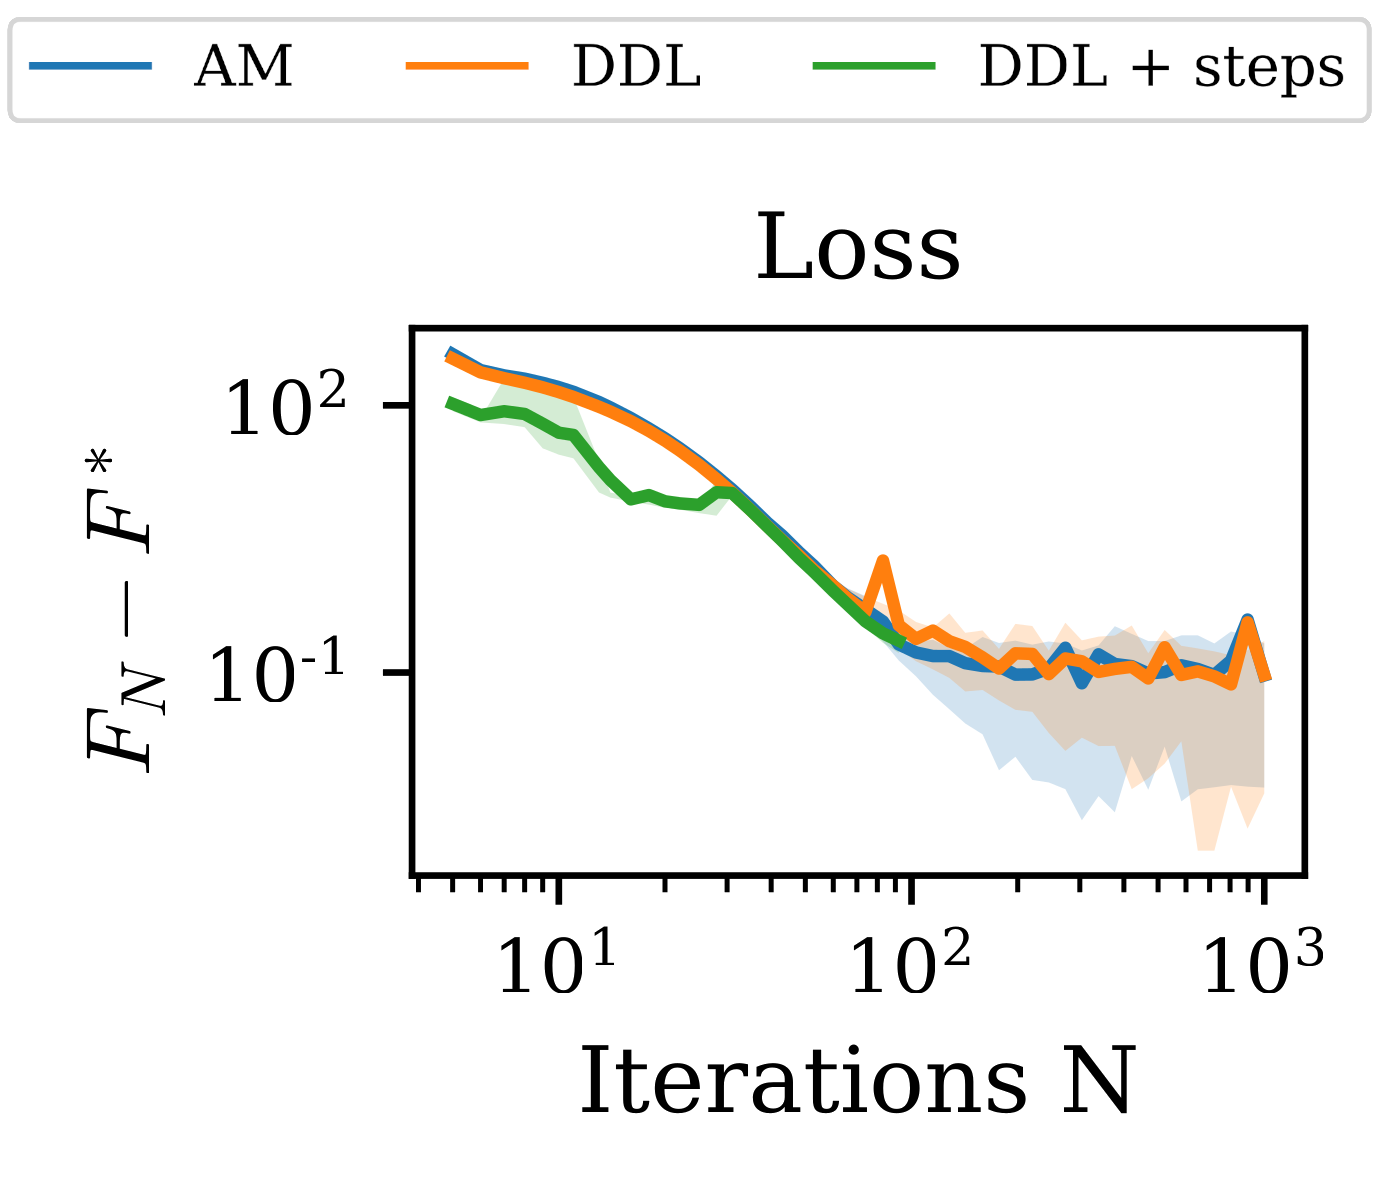
\includegraphics[width=\textwidth]{optim_path.png}\\}
    \end{columns}

    \vskip1em
    \strongpoint{Small number of iterations + learning step size improves uppon AM.}
    % \vskip1em\pause
    % \strongpoint{Not very impressive performance boost.}
}


\frame{
    \frametitle{Unrolling for dictionary learning}

    \vskip4em
    {\centering\bf Not the expected performance boost.\\[2em]}

    \begin{itemize}\itemsep.5em
        \item Jacobian estimate stable only for a low number of iteration.
        \item Possible to design better dictionary learning algorithms but need extra ingredients.
        \item Maybe useful for task-driven dictionary learning.
    \end{itemize}

    \vspace{0pt plus 1 filll}
    \footnotesize
    We are currently investigating the interplay between $G$ and the learning of $D$.

}



\frame{
    \frametitle{Other interest}

    {\bf Bi-level optimization}\\[.5em]
    \begin{itemize}\itemsep.5em
        \item Faster solver for DEQ (SHINE) \contrib{Ramzi et al., ICLR 2022}
        \item Automatic data-augmentation \contrib{Rommel et al., ICLR 2022}
        \item Stochastic solvers \contrib{Dagréou et al., submitted 2022}
    \end{itemize}
    \vskip1em

    {\bf Machine Learning for physiological signals}\\[.5em]
    \begin{itemize}\itemsep.5em
        \item Convolutional Dictionary Learning
        \keypoint{\small[{\color{linkcolor} Moreau et al., ICML 2018}}\\
        \keypoint{\small{\color{linkcolor} Dupre la Tour et al., NeurIPS 2018}]}
        \item Event-based signal processing \contrib{Allain et al., ICLR 2022}
    \end{itemize}
    \vskip1em

    {\bf Open Source Software contributor and maintainer}\\[.5em]
    {\centering
        \includegraphics[height=3em]{logo_python}\hskip2ex
        \includegraphics[height=3em]{logo_sklearn}\hskip2ex
        \includegraphics[height=3em]{logo_joblib}\hskip2ex
        \includegraphics[height=3em]{logo_loky}\hskip2ex
        \includegraphics[height=3em]{logo_benchopt}
        \\[2em]
    }
}

\frame{
    \frametitle{Benchopt: Reproducible, efficient and collaborative
                optimization benchmarks \contrib{Moreau et al., 2022}}

    {\centering 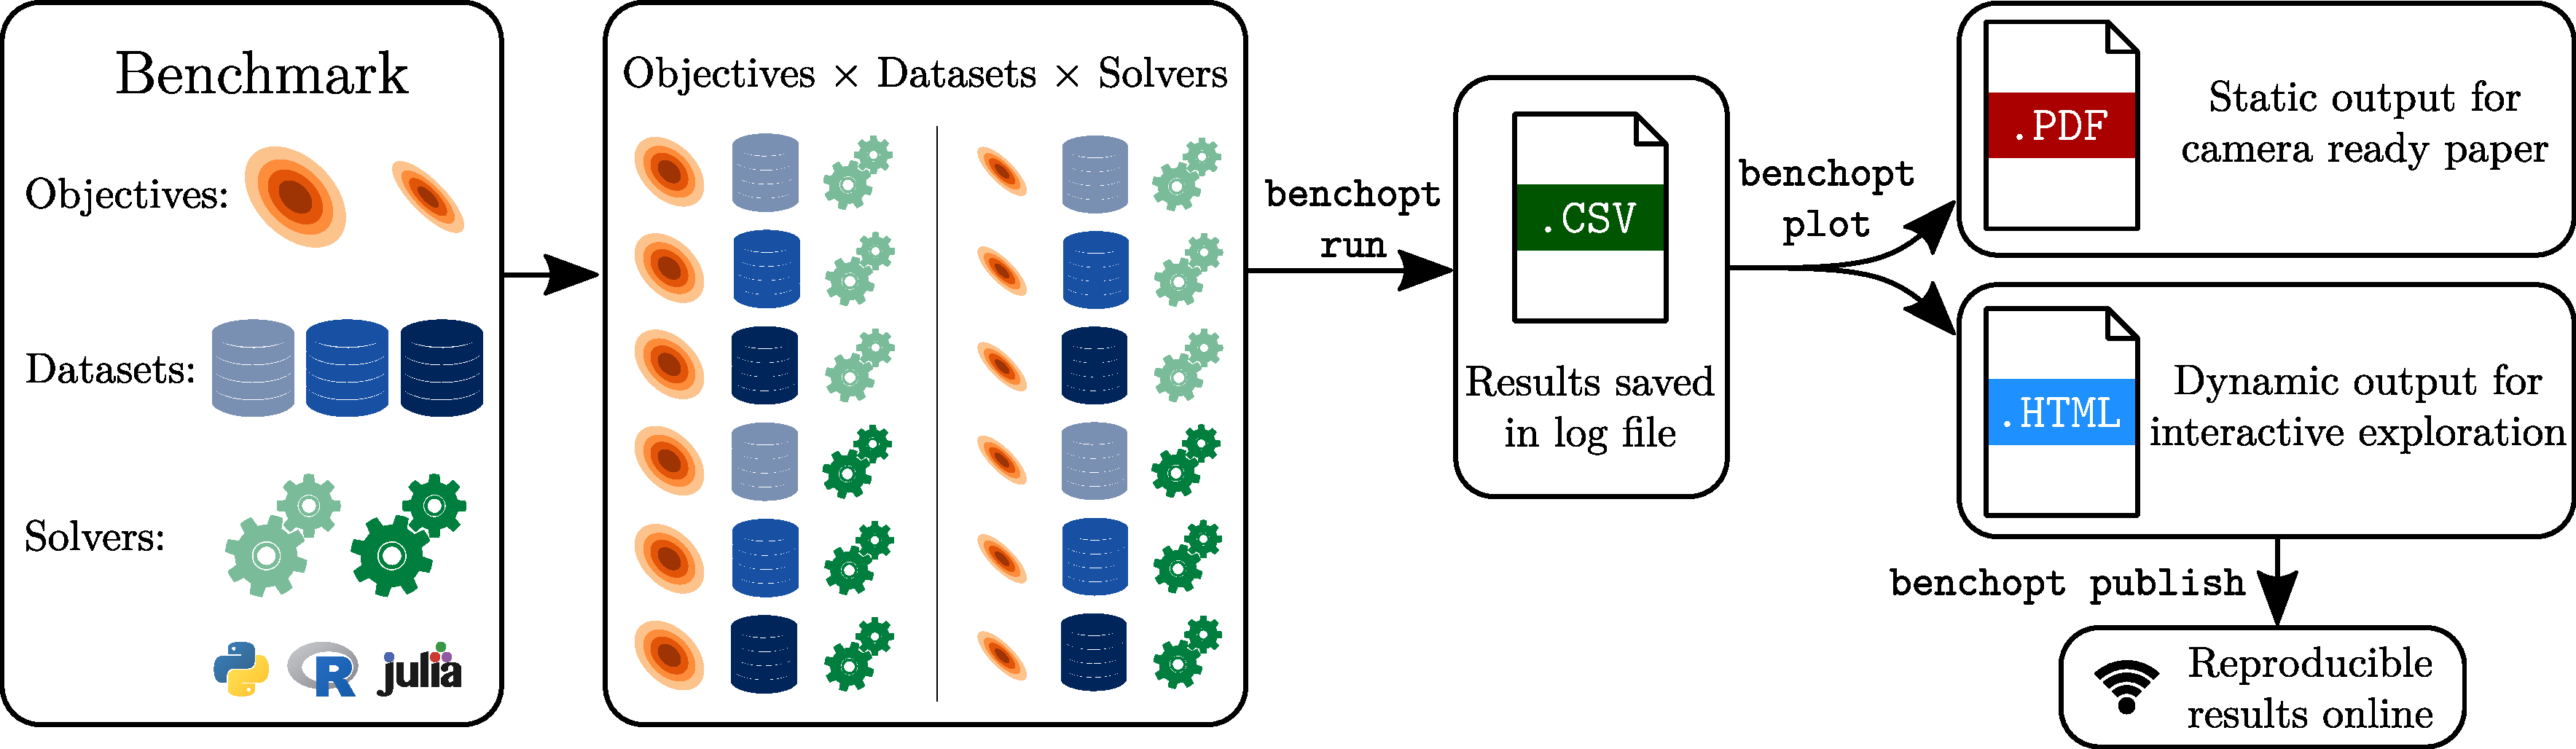
\includegraphics[width=.7\textwidth]{benchopt_schema_objectives_with_logos}\\[1em]

    \url{https://benchopt.github.io/}\\[1em]}

    {\centering
    \raisebox{-1em}{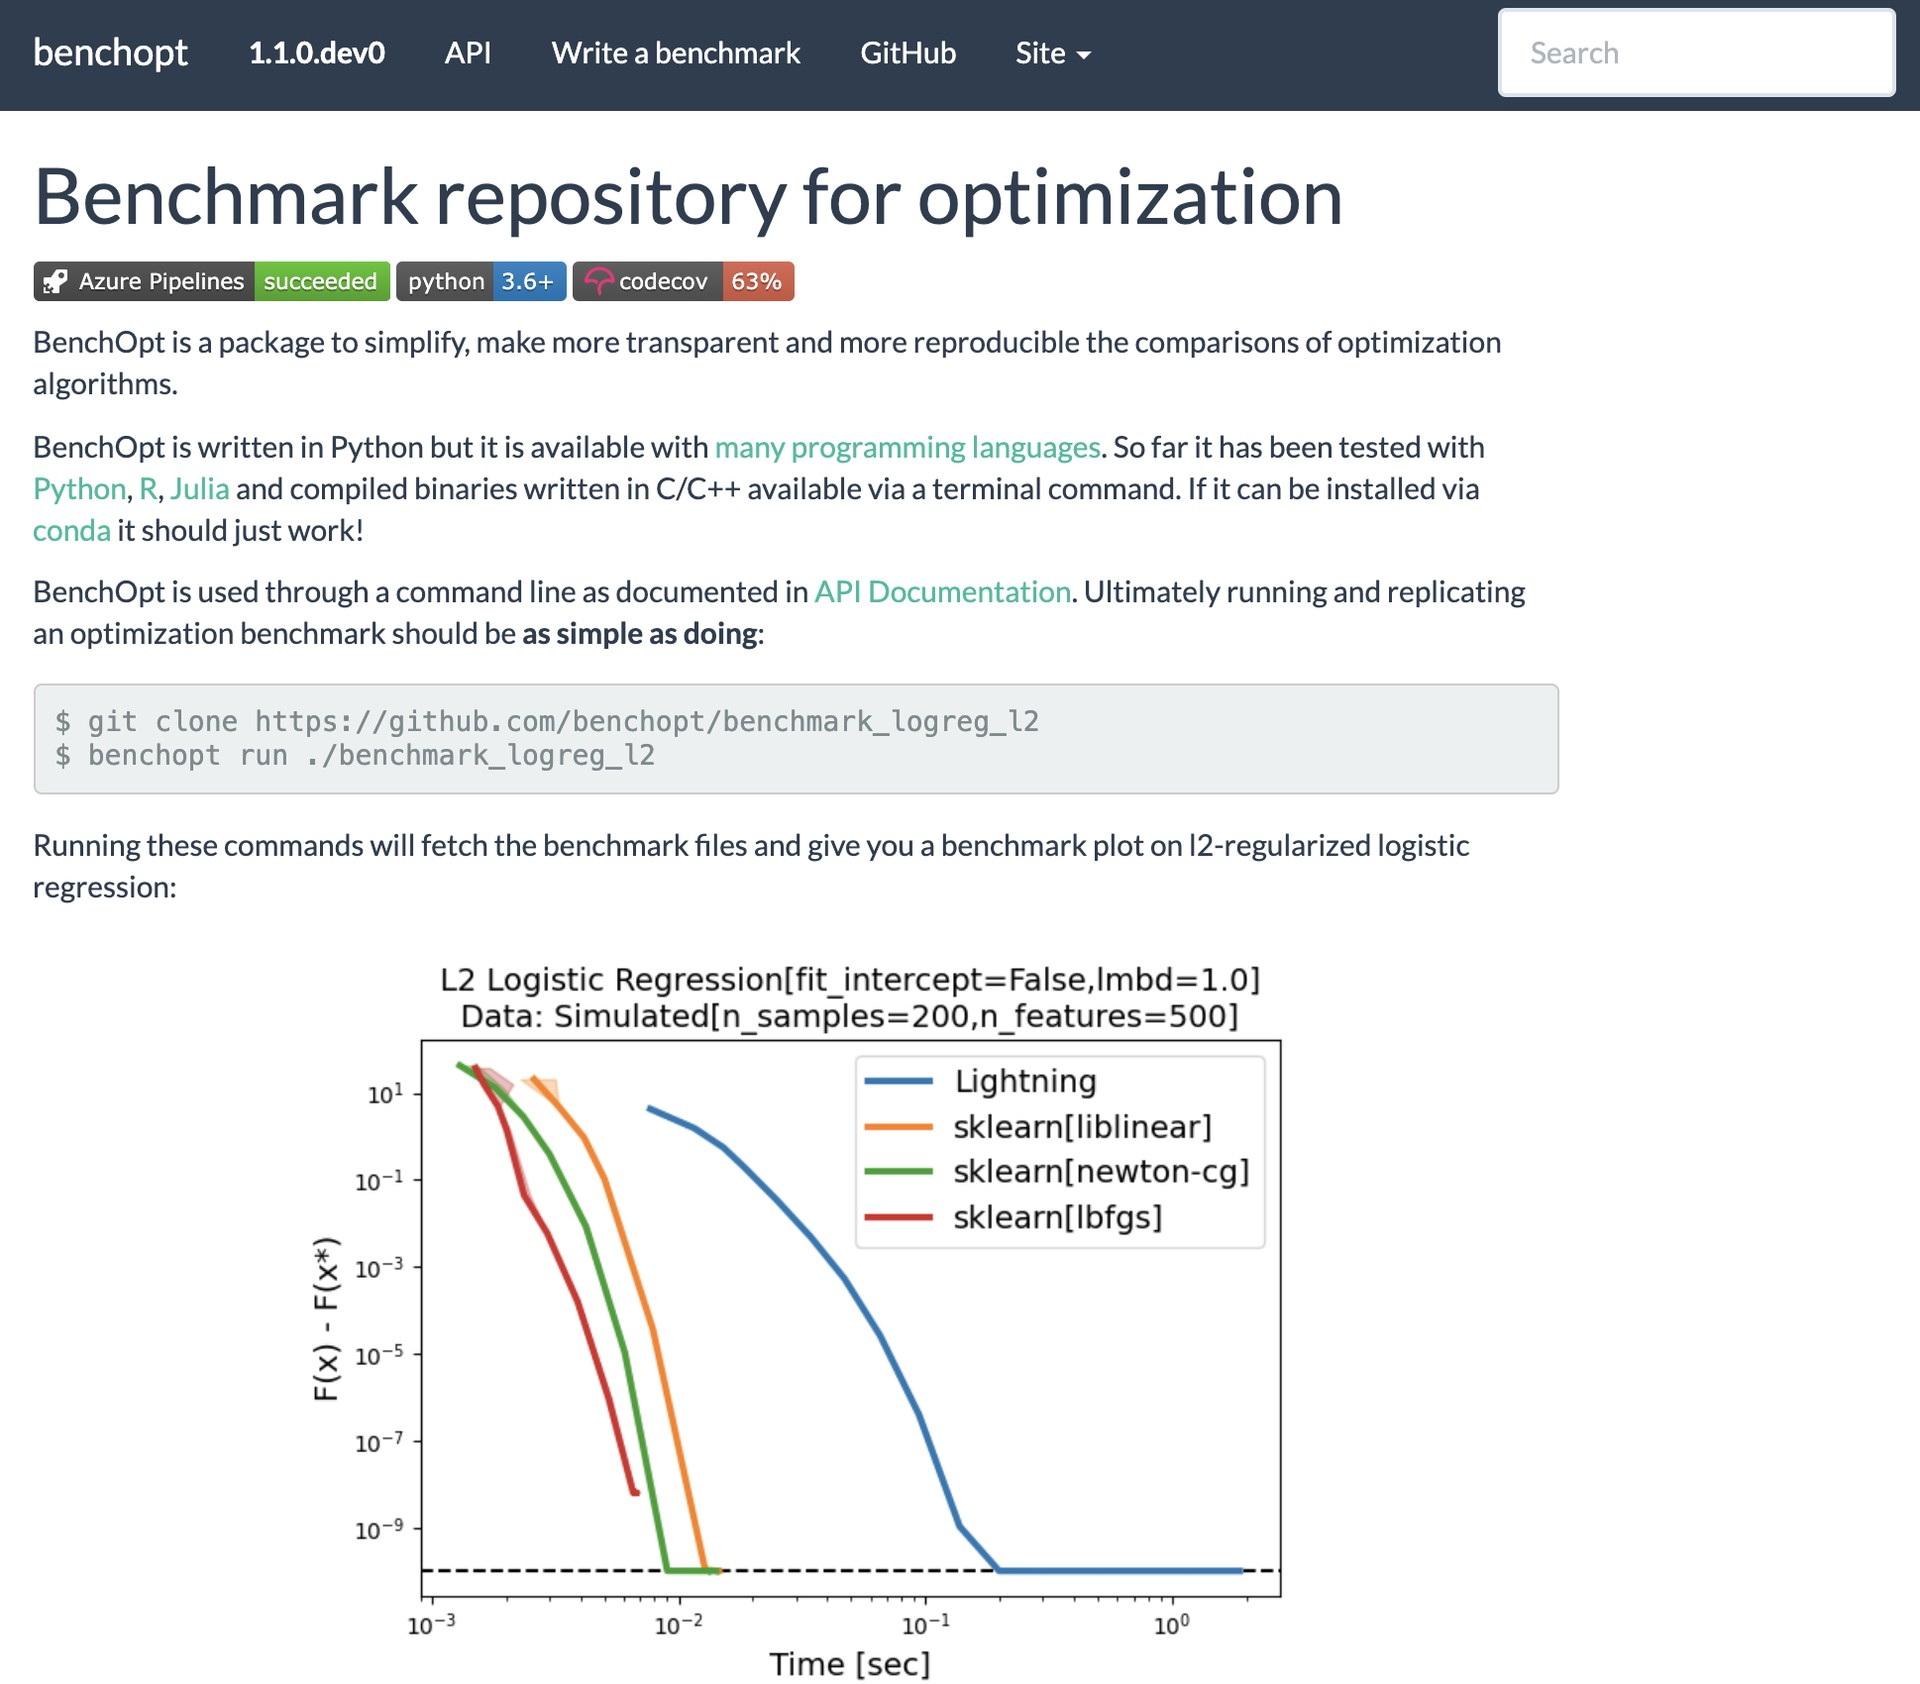
\includegraphics[width=.3\textwidth]{benchopt}}\hskip2ex
    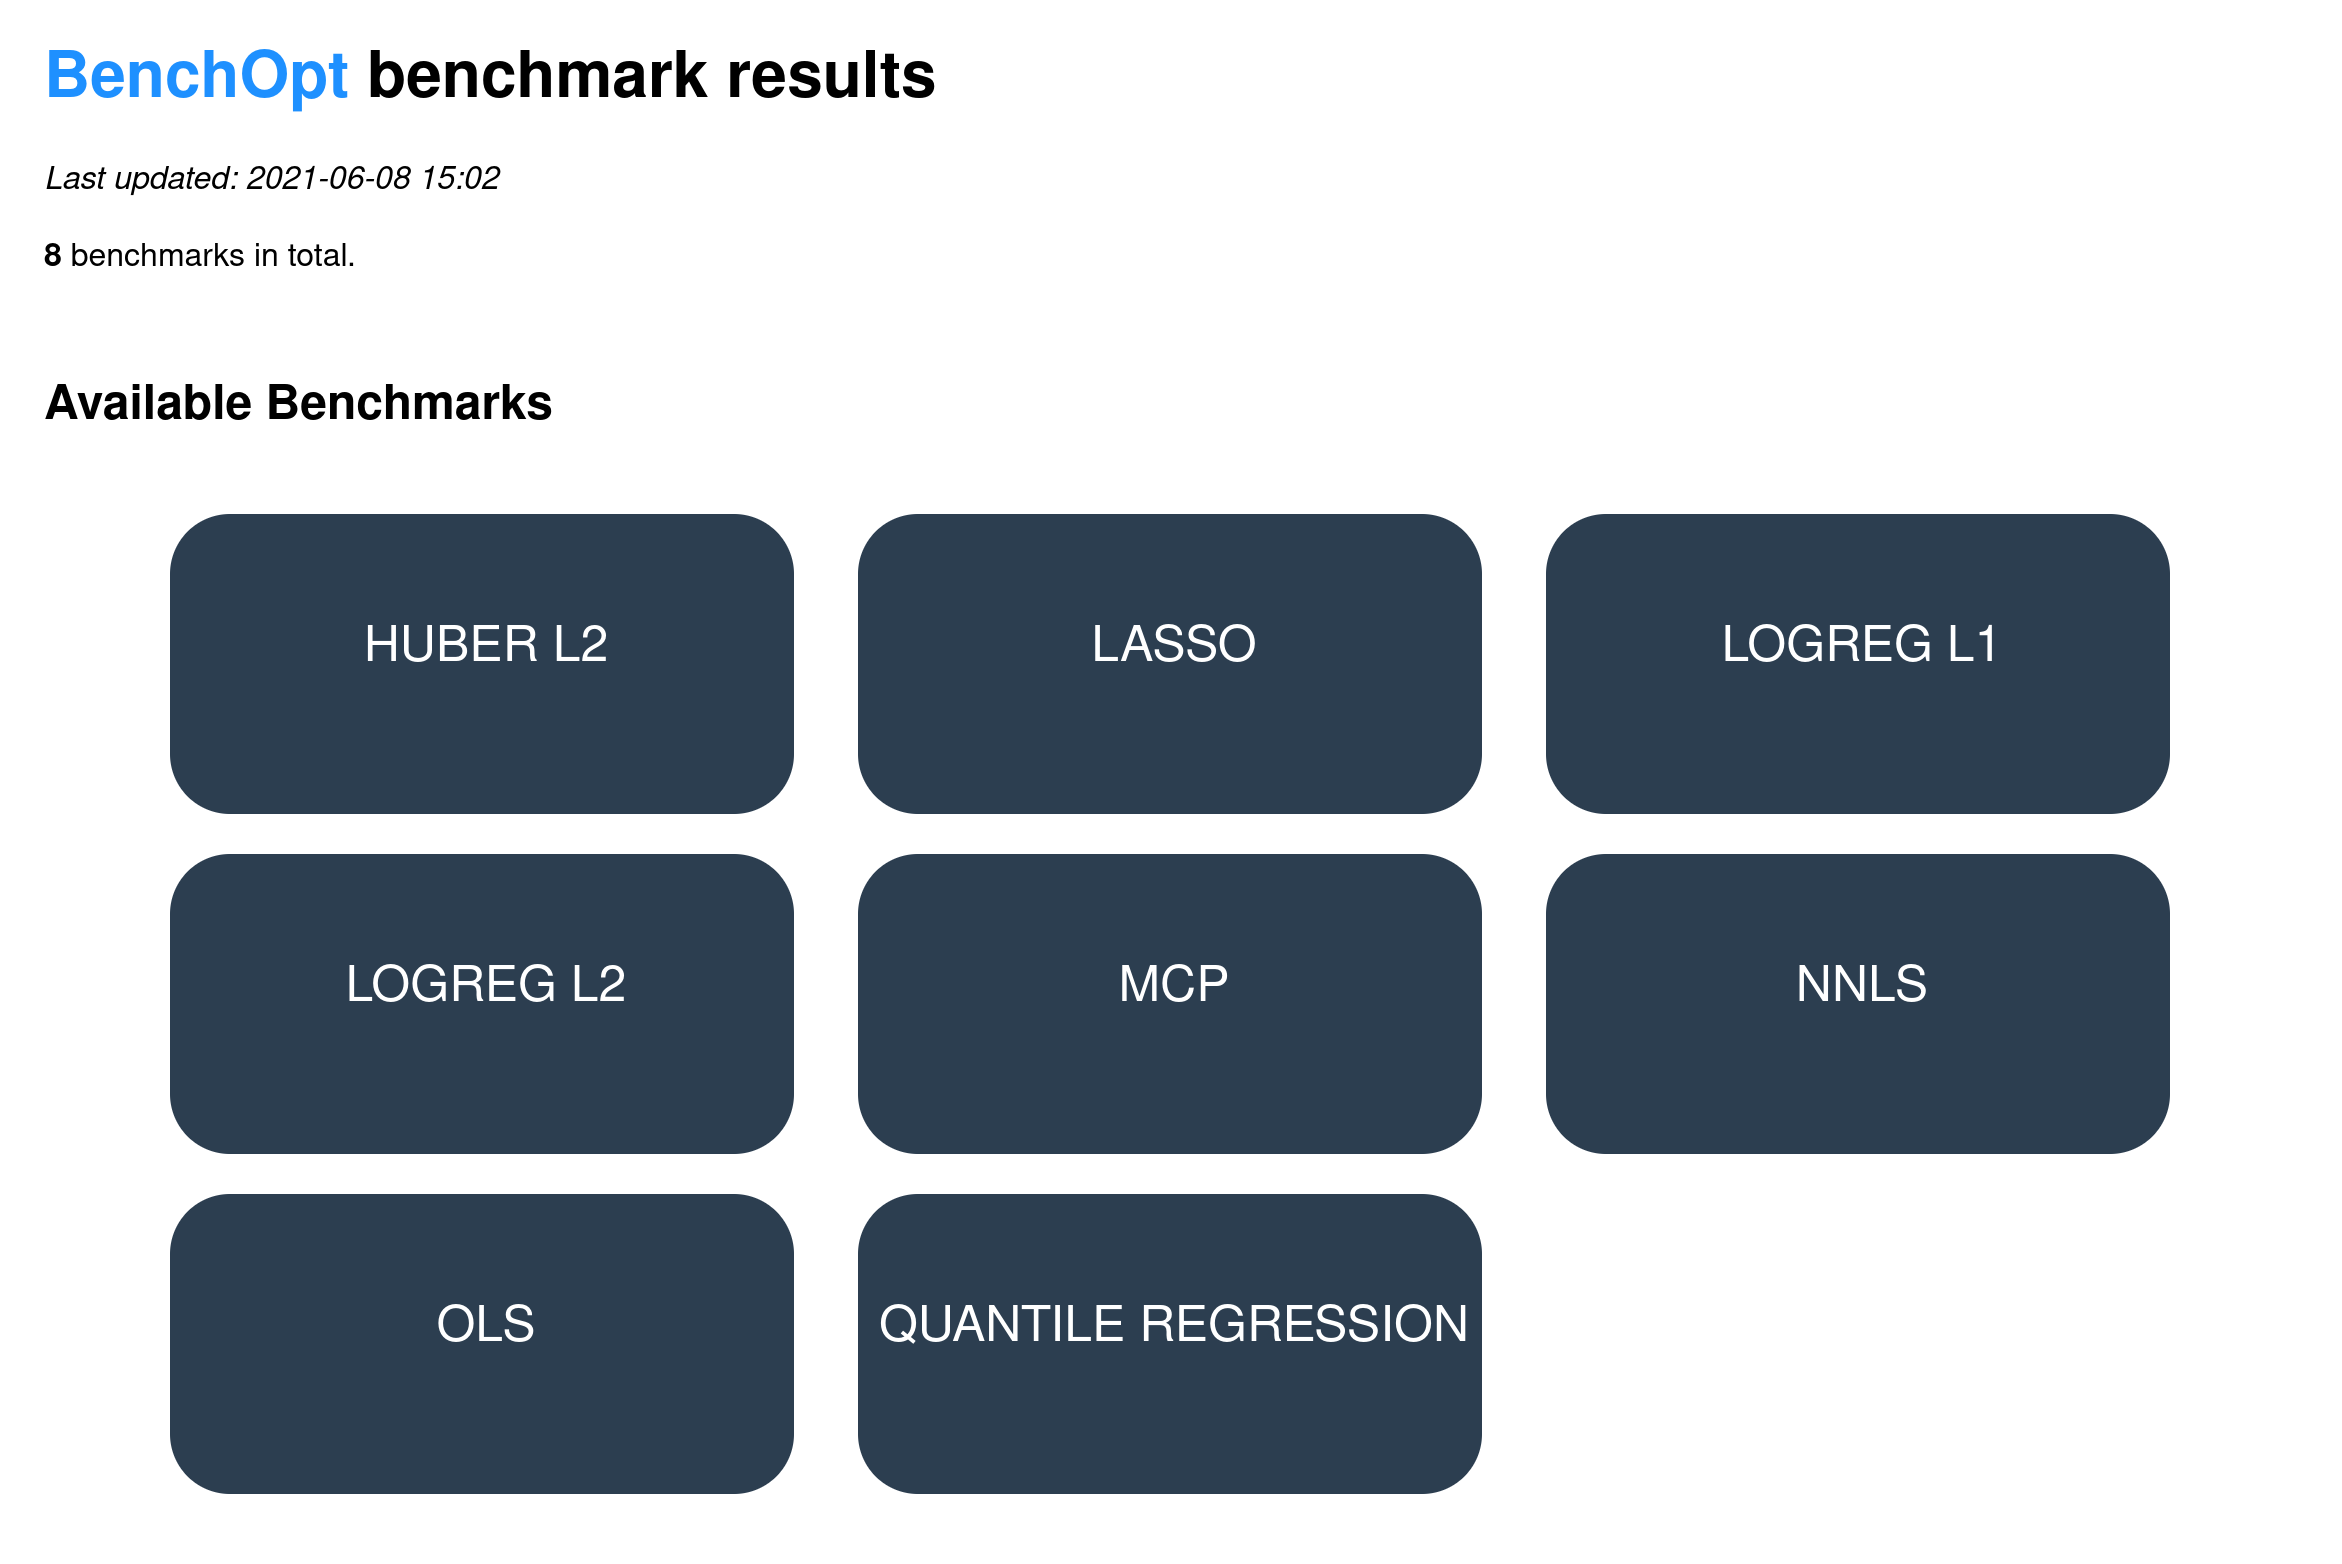
\includegraphics[width=.3\textwidth]{benchopt_results}\hskip2ex
    \raisebox{-1.25em}{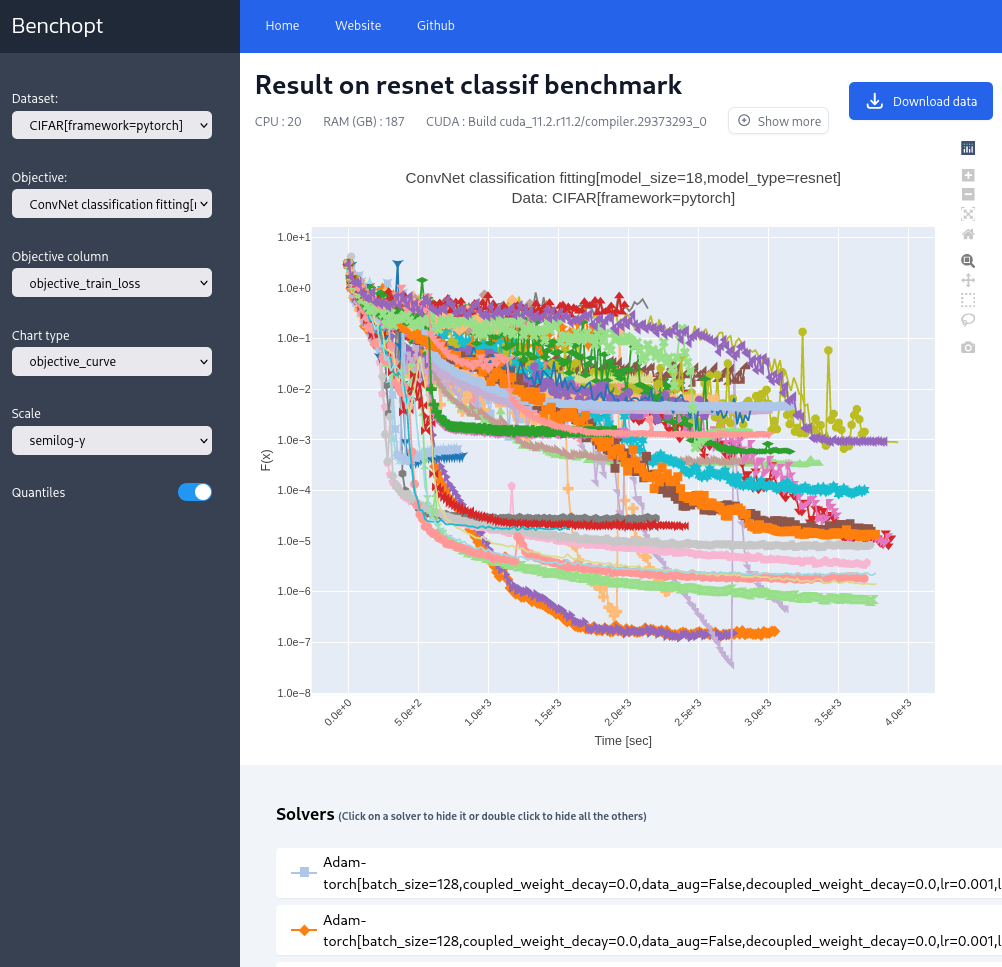
\includegraphics[width=.3\textwidth]{benchopt_convnet}}\\}


}

\frame{
    \vskip2em
    {\centering
        \usebeamercolor[fg]{title}
        \usebeamerfont{title}
        \Huge \bf Thanks for your attention!\\[2em]}

    Slides are on my web page:\\[1em]
    \hskip5em\includegraphics[height=.8em]{website} tommoral.github.io
    \hskip4em 
\includegraphics[height=.8em]{twitter} @tomamoral

}



\appendix


\begin{frame}[t]{ISTA: Majoration-Minimization}
    Taylor expansion of $f_x$ in $z^{(t)}$
    \begin{align*}
        F_x(z) &  = f_x(z^{(t)}) + \nabla f_x(z^{(t)})^\top(z - z^{(t)})
                    + \frac{1}{2}\|D(z-z^{(t)})\|_2^2+ \lambda\|z\|_1\\
               & \le f_x(z^{(t)}) + \nabla f_x(z^{(t)})^\top(z - z^{(t)}) + \frac{L}{2}\|z - z^{(t)}\|_2^2 + \lambda\|z\|_1
    \end{align*}
    $\Rightarrow$ Replace the Hessian $D^\top D$ by $L \textbf{ Id}$.\\[2em]

    Separable function that can be minimized in close form
    \begin{align*}
        \argmin_z \frac{L}{2}\left\|z^{(t)} - \frac{1}{L}\nabla f_x(z^{(t)}) - z\right\|_2^2 + \lambda\|z\|_1
        & = \text{ST}\left(z^{(t)} - \frac{1}{L}\nabla f_x(z^{(t)}),
                           \frac{\lambda}{L}\right)\\
        & = \text{prox}_{\frac{\lambda}{L}}\left(z^{(t)} - \frac{1}{L}\nabla f_x(z^{(t)})\right)
    \end{align*}
\end{frame}

\begin{frame}{ISTA: Majoration for the data-fit}
    \definecolor{darkgreen}{RGB}{0, 148, 0}
    \myitem{} Level lines form $z^\top D^\top D z
                       \only<2>{\le \color{red} L \|z\|_2}
                       \only<3>{\le \color{blue} z^\top A^\top \Lambda A z}
                       \only<4>{\le {\color{darkgreen} L_S \|z\|_2}
                            ~~ \text{ for } Supp(z) \subset S}$
              \only<3>{\contrib{Moreau and Bruna, 2017}}\\
    \centering
    \makebox[.75\textwidth][c]{
        \only<1>{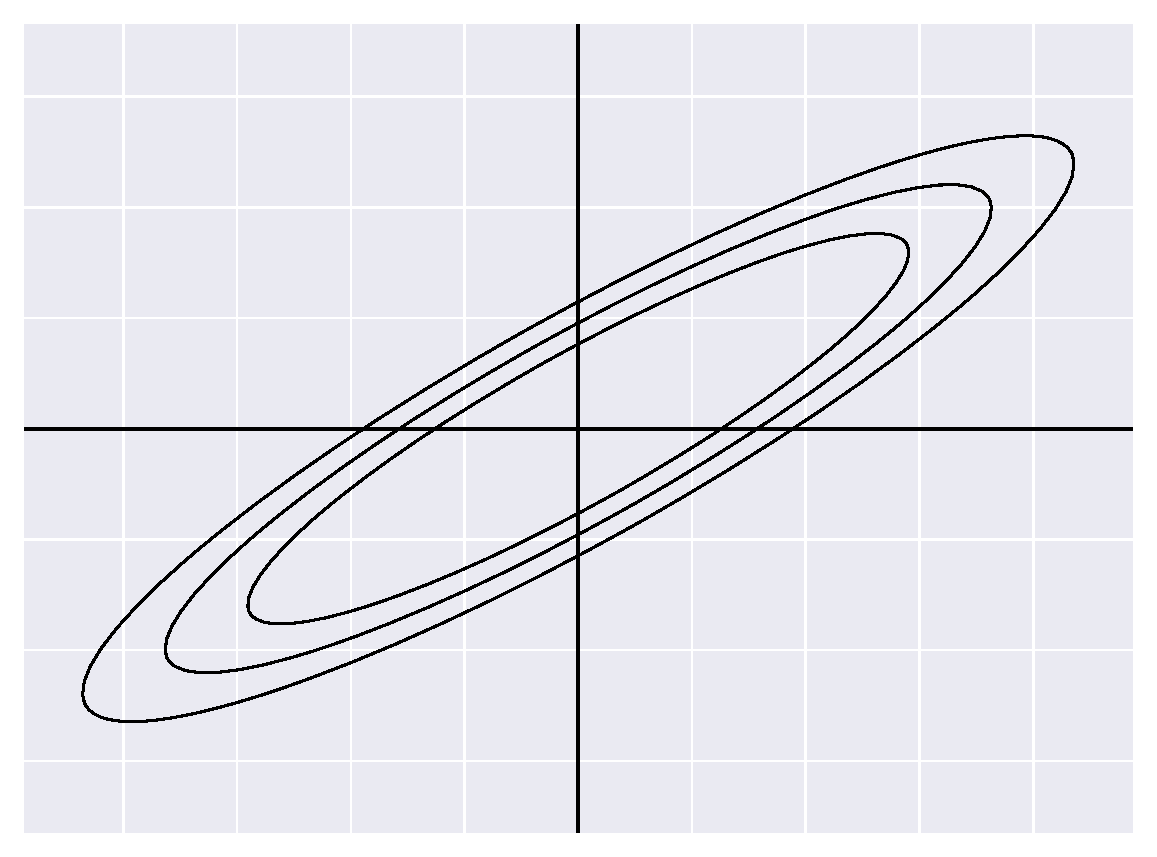
\includegraphics[height=.75\textheight]{ell1}}%
        \only<2>{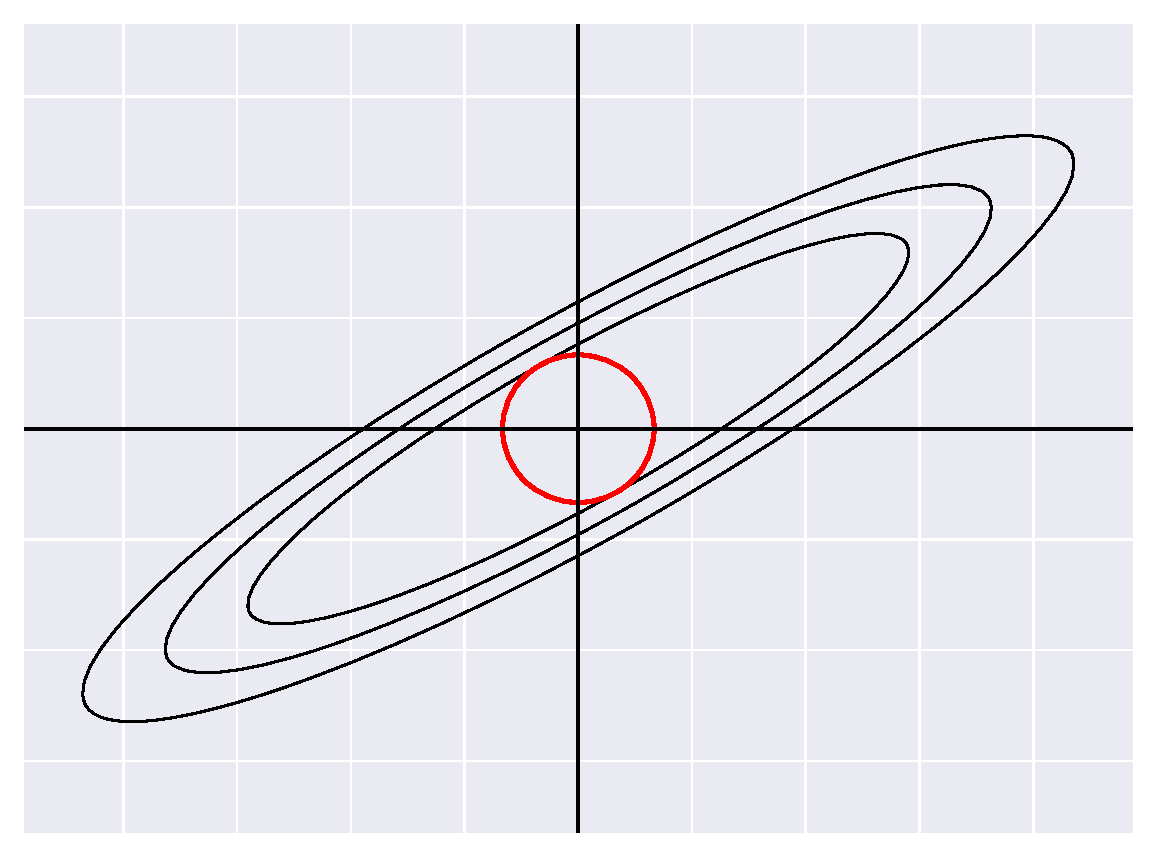
\includegraphics[height=.75\textheight]{ell2}}%
        \only<3>{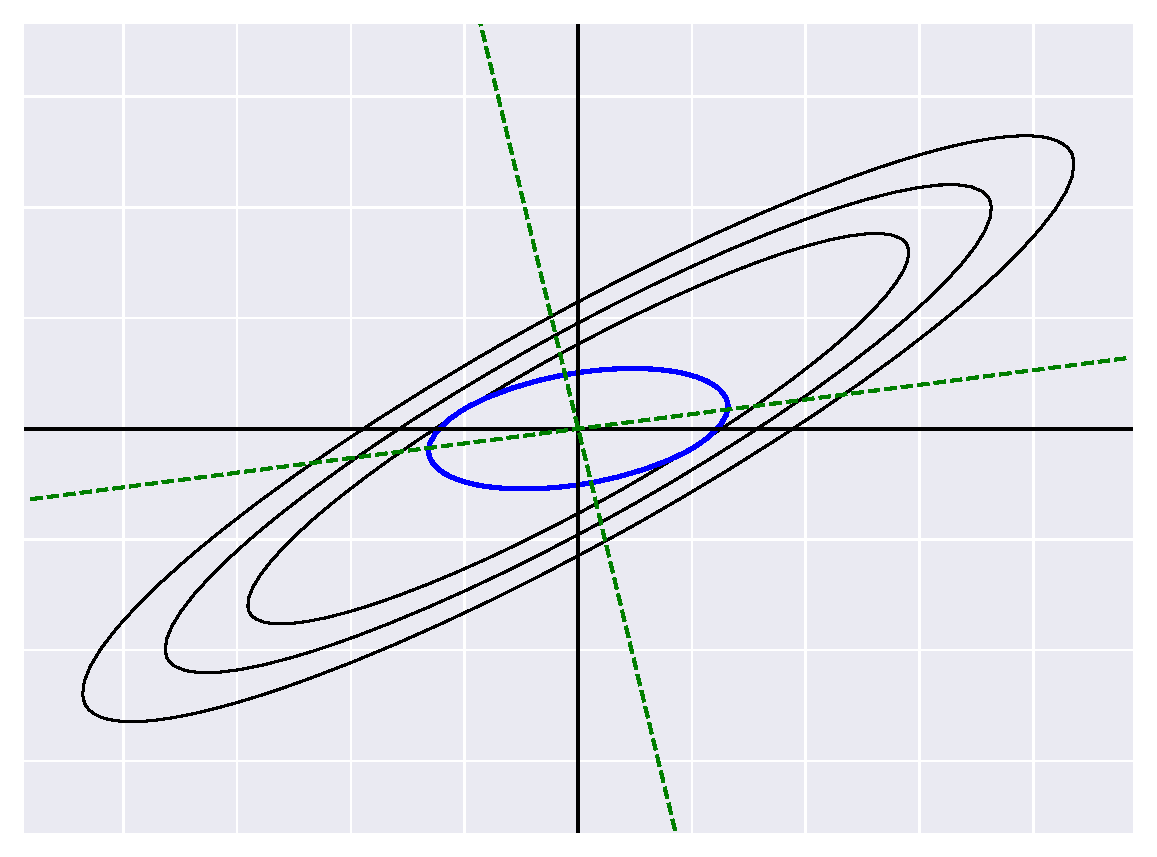
\includegraphics[height=.75\textheight]{ell3}}%
        \only<4>{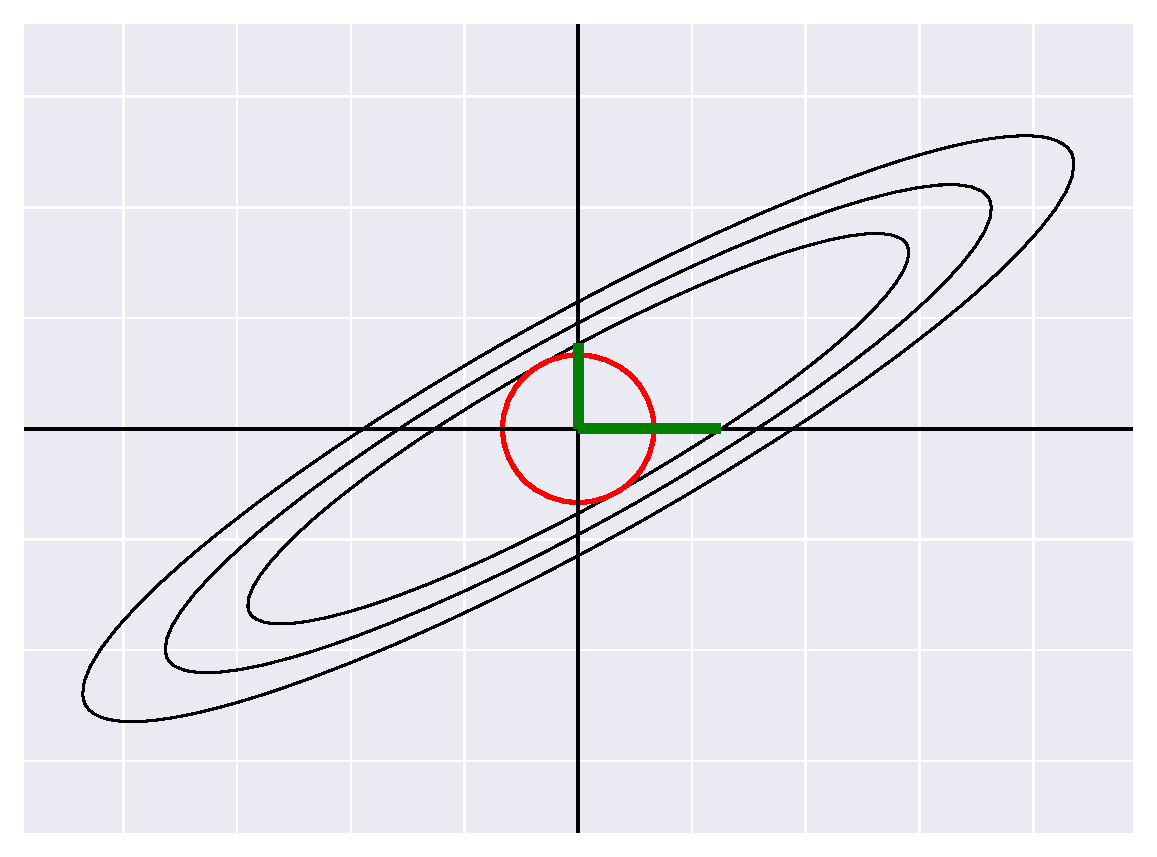
\includegraphics[height=.75\textheight]{ell4}}
    }\\
\end{frame}


\frame{
    \frametitle{Convolutional Dictionary Learning for MEG}

    {\bf Learning waveforms from MEG recordings}\\[1em]
    {\centering
    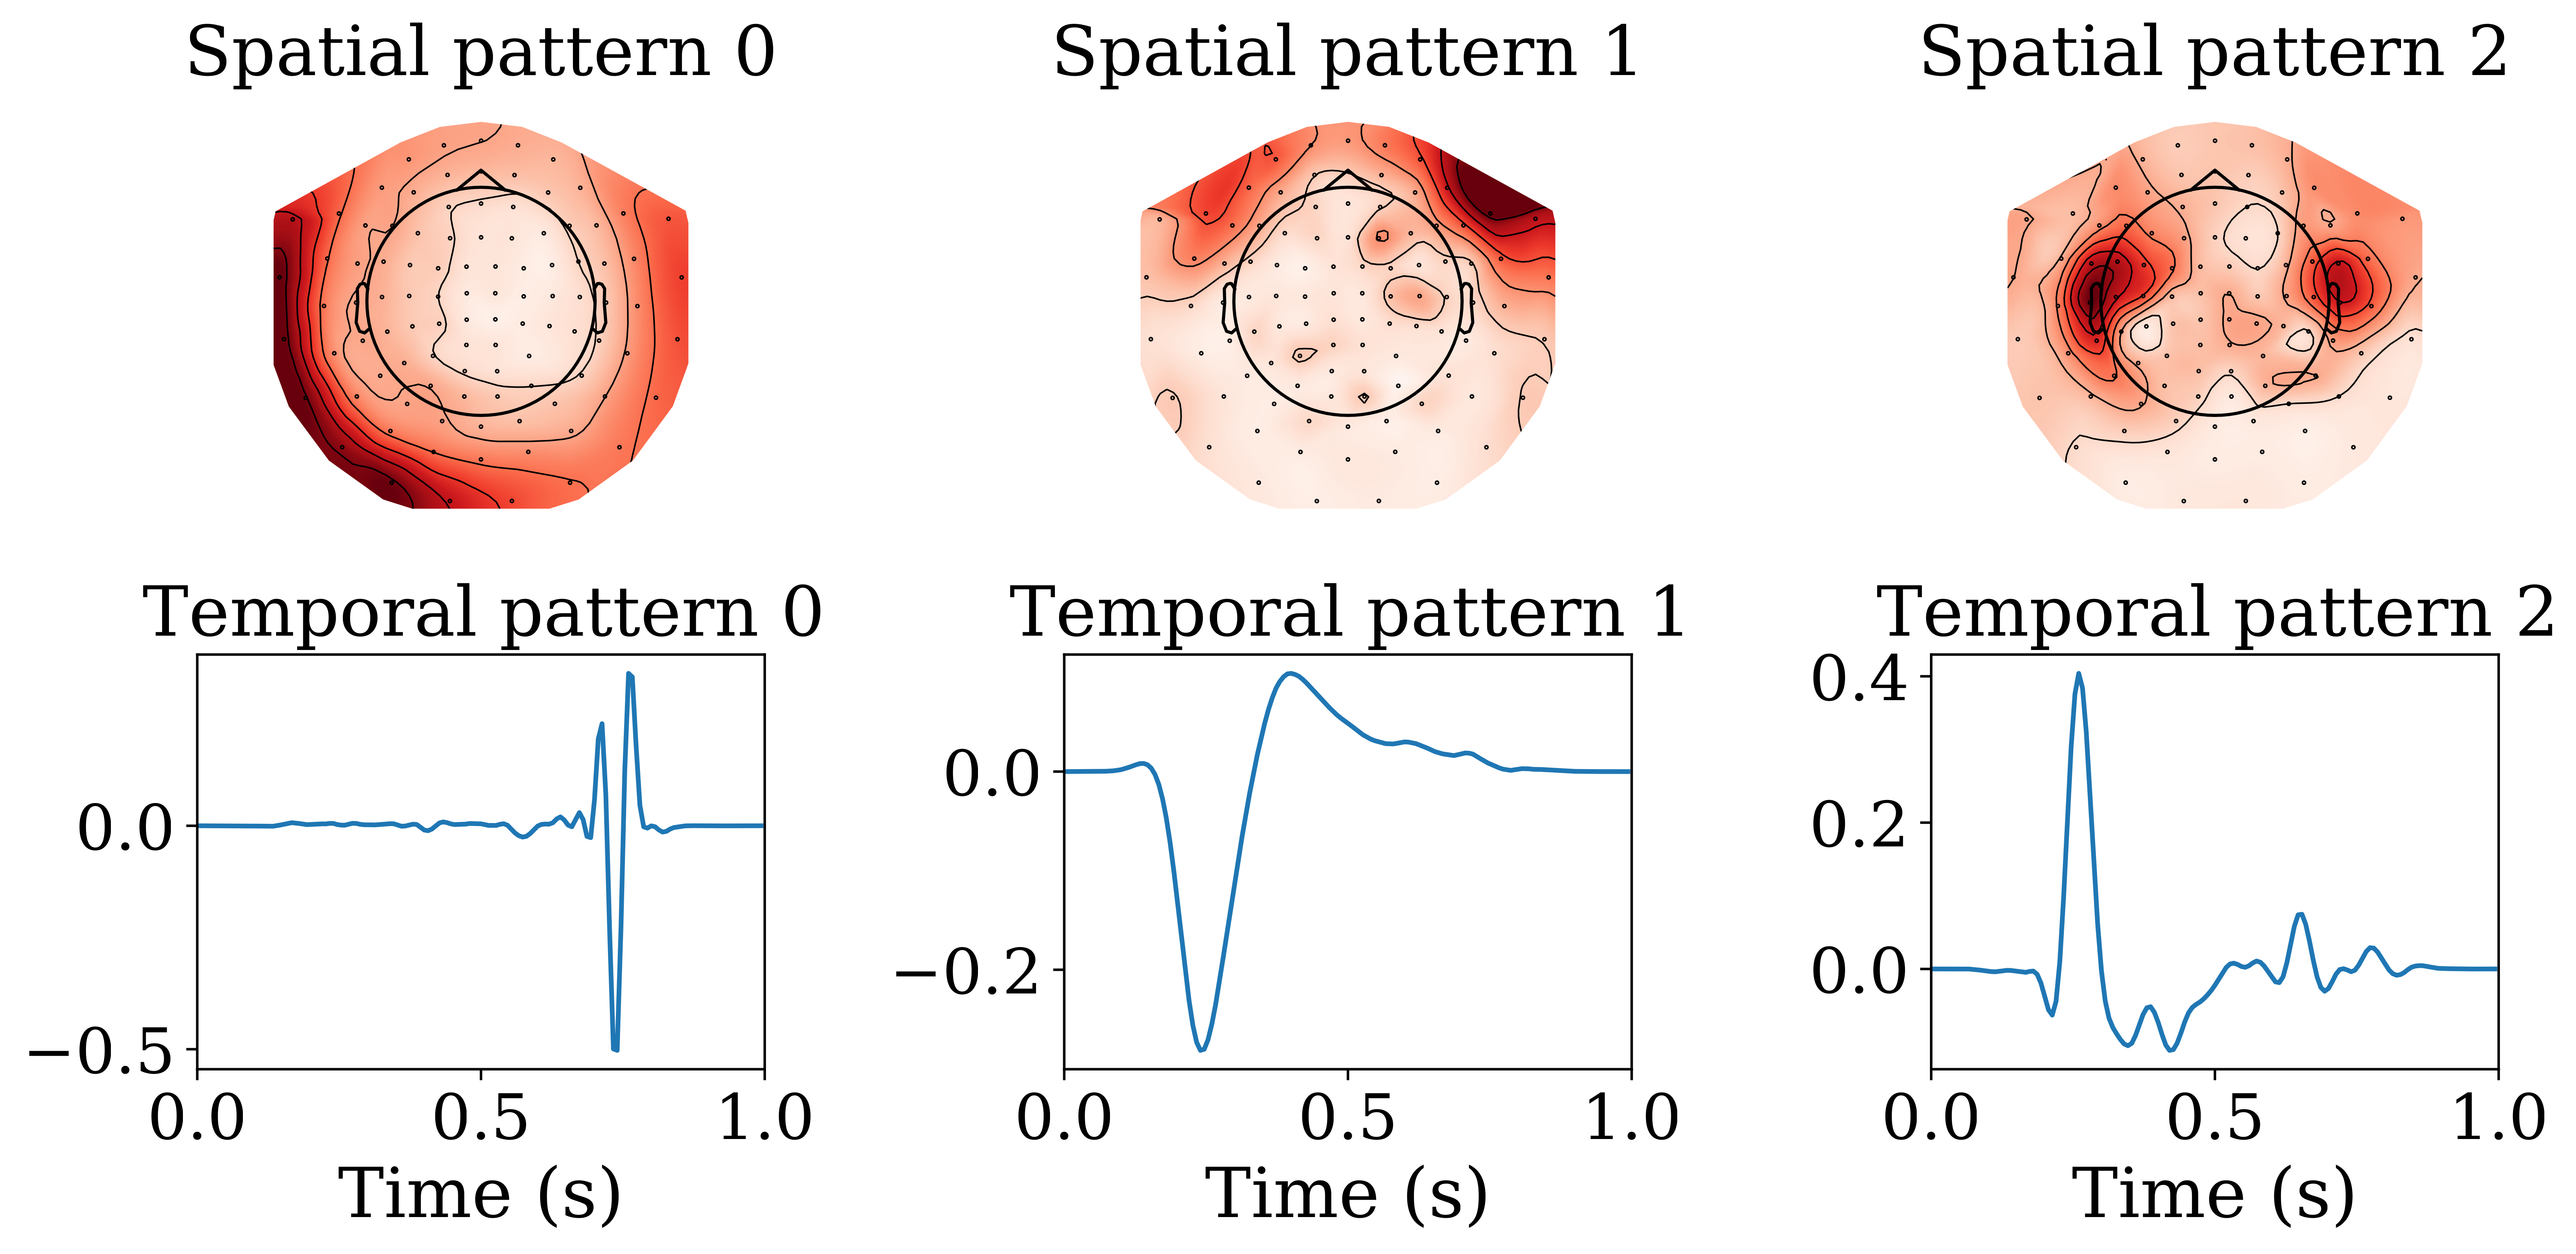
\includegraphics[width=.8\textwidth]{meg_figure.png}\\[2em]}

    DDL + stochastic $\sim$ 150s\\
    \texttt{alphacsc} $\sim$ 1500s \mycite{DuprelaTour2018}\\
    Correlation: between 0.8 and 0.9

}

\frame[t]{
	\frametitle{Local structure in signals}

	\visible<5->{
		\textbf{Key idea}: decouple the localization of the
							patterns and their shape}
    \vskip.5em%
    \centering%
    \only<1>{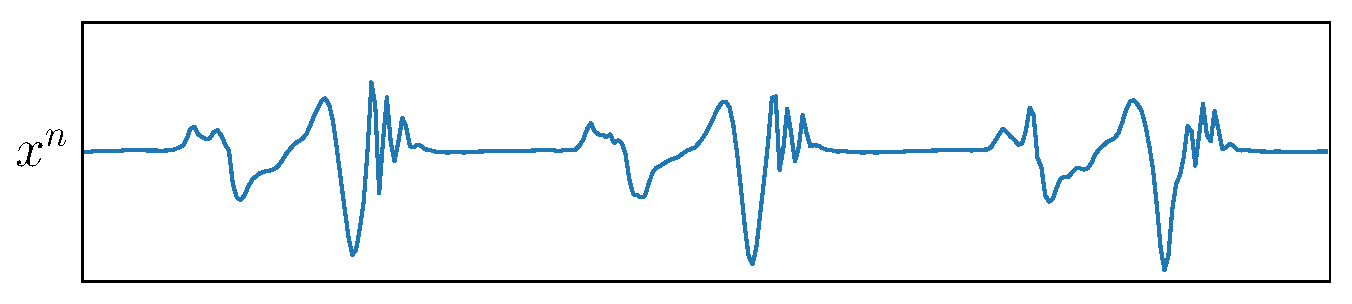
\includegraphics[width=\textwidth]{intro_csc_0}}%
    \only<2>{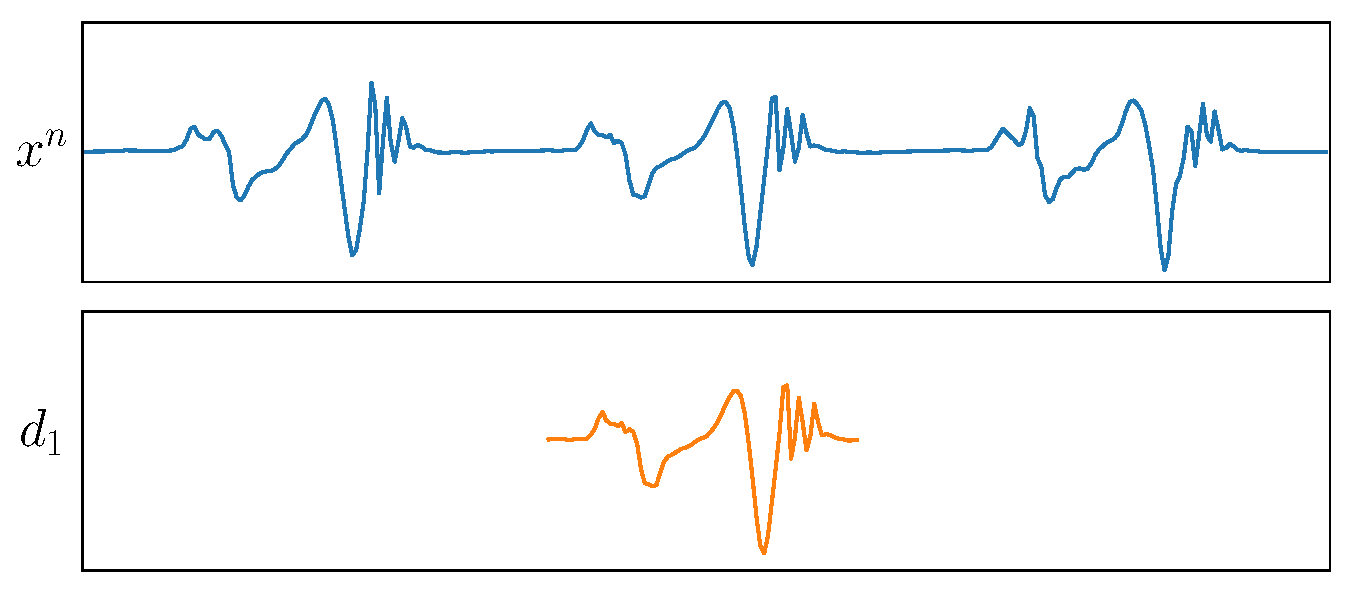
\includegraphics[width=\textwidth]{intro_csc_1}}%
    \only<3>{\includegraphics[width=\textwidth]{intro_csc_2}}%
    \only<4>{\includegraphics[width=\textwidth]{intro_csc_3}}%
    \only<5>{\includegraphics[width=\textwidth]{intro_csc_4}}%
    \only<6->{\includegraphics[width=\textwidth]{intro_csc_5}}%
    \vskip0em%
    \only<7>{%
        \includegraphics[width=.6\textwidth]{csc_explain_eq_color}%
    }
}

\end{document}
